%% Copernicus Publications Manuscript Preparation Template for LaTeX Submissions
%% ---------------------------------
%% This template should be used for copernicus.cls
%% The class file and some style files are bundled in the Copernicus Latex Package, which can be downloaded from the different journal webpages.
%% For further assistance please contact Copernicus Publications at: production@copernicus.org
%% https://publications.copernicus.org/for_authors/manuscript_preparation.html


%% Please use the following documentclass and journal abbreviations for discussion papers and final revised papers.

%% 2-column papers and discussion papers
\documentclass[journal abbreviation, manuscript]{copernicus}



%% Journal abbreviations (please use the same for discussion papers and final revised papers)


% Advances in Geosciences (adgeo)
% Advances in Radio Science (ars)
% Advances in Science and Research (asr)
% Advances in Statistical Climatology, Meteorology and Oceanography (ascmo)
% Annales Geophysicae (angeo)
% Archives Animal Breeding (aab)
% ASTRA Proceedings (ap)
% Atmospheric Chemistry and Physics (acp)
% Atmospheric Measurement Techniques (amt)
% Biogeosciences (bg)
% Climate of the Past (cp)
% DEUQUA Special Publications (deuquasp)
% Drinking Water Engineering and Science (dwes)
% Earth Surface Dynamics (esurf)
% Earth System Dynamics (esd)
% Earth System Science Data (essd)
% E&G Quaternary Science Journal (egqsj)
% European Journal of Mineralogy (ejm)
% Fossil Record (fr)
% Geochronology (gchron)
% Geographica Helvetica (gh)
% Geoscience Communication (gc)
% Geoscientific Instrumentation, Methods and Data Systems (gi)
% Geoscientific Model Development (gmd)
% History of Geo- and Space Sciences (hgss)
% Hydrology and Earth System Sciences (hess)
% Journal of Micropalaeontology (jm)
% Journal of Sensors and Sensor Systems (jsss)
% Mechanical Sciences (ms)
% Natural Hazards and Earth System Sciences (nhess)
% Nonlinear Processes in Geophysics (npg)
% Ocean Science (os)
% Primate Biology (pb)
% Proceedings of the International Association of Hydrological Sciences (piahs)
% Scientific Drilling (sd)
% SOIL (soil)
% Solid Earth (se)
% The Cryosphere (tc)
% Weather and Climate Dynamics (wcd)
% Web Ecology (we)
% Wind Energy Science (wes)


%% \usepackage commands included in the copernicus.cls:
%\usepackage[german, english]{babel}
\usepackage{tabularx}
%\usepackage{cancel}
\usepackage{multirow}
%\usepackage{supertabular}
%\usepackage{algorithmic}
%\usepackage{algorithm}
%\usepackage{amsthm}
%\usepackage{float}
%\usepackage{subfig}
%\usepackage{rotating}

\usepackage{booktabs}
%\usepackage{ltablex}

\begin{document}

\title{Evaluation of climate model aerosol trends with ground-based observations over the last two decades - an AeroCom and CMIP6 analysis}


% \Author[affil]{given_name}{surname}
\Author[1]{Augustin}{Mortier}
\Author[1]{Jonas}{Gliss}
\Author[1]{Michael}{Schulz}
%alphabetical after here
\Author[2]{Wenche}{Aas}
\Author[3]{Elisabeth}{Andrews}
\Author[4]{Huisheng}{Bian}
\Author[5]{Mian}{Chin}
\Author[6]{Paul}{Ginoux}
\Author[7]{Jenny}{Hand}
\Author[5]{Brent}{Holben}
\Author[8]{Zhang}{Hua}
\Author[9]{Zak}{Kipling}
\Author[1]{Alf}{Kirkevåg}
\Author[10]{Gunnar}{Myhre}
\Author[11]{David}{Neubauer}
\Author[1]{Dirk}{Olivié}
\Author[12]{Toshihiko}{Takemura}


\affil[1]{Norwegian Meteorological Institute, Oslo, Norway}
\affil[2]{NILU, Norwegian Institute for Air Research, Kjeller, Norway}
\affil[3]{Cooperative Institute for Research in Environmental Sciences,University of Colorado, Boulder, Colorado, USA}
\affil[4]{Maryland Univ. Baltimore County (UMBC), Baltimore, MD, USA}
\affil[5]{NASA Goddard Space Flight Center, Greenbelt, Maryland, USA}
\affil[6]{NOAA, Geophysical Fluid Dynamics Laboratory, Princeton, NJ, USA}
\affil[7]{Cooperative Institute for Research in the Atmosphere, Colorado State University, Fort Collins, CO, USA}
\affil[8]{Laboratory for Climate Studies, National Climate Center,
China Meteorological Administration, Beijing, China}
\affil[9]{European Centre for Medium-Range Weather Forecasts, Reading, UK}
\affil[10]{CICERO Center for International Climate and Environmental Research, Oslo, Norway}
\affil[11]{Institute for Atmospheric and Climate Science, ETH Zurich, Zurich, Switzerland}
\affil[12]{Research Institute for Applied Mechanics, Kyushu University, 6-1 Kasuga-koen, Kasuga, Fukuoka, Japan}


%co-authors/references:
%CanESM5: ?
%CESM2: ?
%IPSL-CM6A: ?




%% The [] brackets identify the author with the corresponding affiliation. 1, 2, 3, etc. should be inserted.
%% If an author is deceased, please add a further affiliation and mark the respective author name(s) with a dagger, e.g. "\Author[2,$\dag$]{Anton}{Aman}" with the affiliations "\affil[2]{University of ...}" and "\affil[$\dag$]{deceased, 1 July 2019}"


\correspondence{Augustin Mortier (augustinm@met.no)}

\runningtitle{Aerosol Trends}

\runningauthor{Augustin Mortier}

\received{}
\pubdiscuss{} %% only important for two-stage journals
\revised{}
\accepted{}
\published{}
%% These dates will be inserted by Copernicus Publications during the typesetting process.


\firstpage{1}

\maketitle

\textcolor{red}{Please check acknowledgements section}

%\tableofcontents

\begin{abstract}
 This study presents a multi-parameter analysis of the aerosol trends over the last two decades at regional and global scales. Regional time series have been computed for a set of nine optical and microphysical properties by using the observations of several ground-based networks. From these regional time series the aerosol trends have been derived for different regions of the world. Most of the extensive properties exhibit negative trends, both at the surface and in the total atmospheric column. Significant decreases of aerosol optical depth (AOD) are found in Europe, North America, South America and North Africa, ranging from -1.3\%/yr to -3.1\%/yr. An error and representativity analysis of the incomplete observational data has been performed using model data subsets in order to investigate how likely the observed trends represent the actual trends happening in the regions over the full study period from 2000 to 2014. This analysis reveals that significant uncertainty is associated with some of the regional trends due to time and space sampling deficiencies. The set of observed regional trends has then been used for the evaluation of the climate models and their skills in reproducing the aerosol trends. Model performance is found to vary depending on the parameters and the regions of the World. The models tend to capture trends in AOD, column Angstrom exponent, sulfate and PM well, but show larger discrepancies for coarse mode AOD. The most robust aerosol trends are found for Europe and North America (-2.9\%/year in AOD). The models can help to provide a global picture of the aerosol trends by filling the gaps in the regions not covered by observations. The calculation of the aerosol trends at a global scale reveals a different picture from the one depicted by solely relying on ground based observations. Using a model with complete diagnostics (NorESM2) we find a global increase of AOD of about 0.2\%/yr between 2000 and 2014, primarily caused by an increase of the loads of organic aerosol, sulfate and black carbon.
\end{abstract}


\copyrightstatement{TEXT}


\introduction  %% \introduction[modified heading if necessary]
As one of the key gears involved in the climate mechanism \citep{poschl2005atmospheric}, and as a predominant component of air quality that affects human health \citep{burnett2014integrated}, aerosols have been increasingly subject to observation over the last two decades, both from ground and space-based platforms \citep{holben2001emerging,kaufman2002satellite}.  Aerosols are also recognized to have an important role for the fertilization of the Amazon forest \citep{yu2015fertilizing}, and in other socioeconomic fields such as the solar energy production \citep{Li11867,labordena2018blue}.

Through their direct, semi-direct and indirect effects \citep{rap2013natural,johnson2004semi,lohmann2005global}, aerosol particles are crucial for the estimation of the radiative forcing. Currently, the overall estimate of aerosol radiative forcing is associated with high uncertainties \citep{haywood2000estimates, stocker2014climate}. Some of the reasons for these uncertainties reside in the heterogeneity of atmospheric particles, both in terms of their microphysical and optical properties, as well as the high variability of these aerosols in space and time. The different regions of the world exhibit contrasting aerosol properties \citep{holben2001emerging}, which can also vary depending on the seasons, or on longer scales \citep{streets2009anthropogenic}. In addition to natural emissions such as sea salt and dust, anthropogenic sources of aerosol add another layer of complexity. The development of countries during the Second Industrial Revolution, which relied on the use of fossil fuel energy, has had a significant impact on the aerosol load on a global scale, and on the local air quality, resulting in severe pollution episodes, such as the famous smog event in London, 1952 \citep{bell2004retrospective} that caused the death of thousands of people within a few days.
Starting in the 1970s mitigation measures were established to limit the emission of particles and other pollutants \citep{bryner1995blue,turnock2016impact} resulting in significant improvements in terms of air quality and particle concentration levels \citep{likens2001long}. There has been a shift of anthropogenic emissions from Europe and North America to the developing nations, which are now facing the major air quality issues that were affecting the Europe and North America 40 years ago \citep{streets2008aerosol,ramachandran2012aerosol}.

In order to provide realistic radiative forcing estimates and projections, it is important for the models to be able to capture the aerosol trends caused by both natural and anthropogenic variations. With a consistent multi-parameter analysis, this study presents an overview of aerosol trends using ground based observation network data as a reference for the evaluation of the models skills in reproducing the aerosols trends.

To serve that purpose, this study addresses the following three questions:
\begin{itemize}
    \item What are the observed aerosol trends over the last two decades in the different regions of the World? (\ref{obs_trends})
    \item Can the climate models reproduce these observed trends? (\ref{mod_evaluation})
    \item What are the global aerosol trends derived from the model data? (\ref{global_trends})
\end{itemize}

Figure \ref{fig:hist_runs} presents the time series of global modeled AOD between 1850 and 2014. All of the climate models appear to capture a large increase, especially between 1950 and 1990, followed by more stable conditions up to the present. The aerosol optical measurements, which started to develop in the late 1990's, allow investigation of the trends over the last two decades, and offer an opportunity to validate the modeled trends in this period. Since 2014 is the last year available from the CMIP6 historical runs, we focus this study on the aerosol trends in the 2000-2014 period.

\begin{figure}
 \centering
 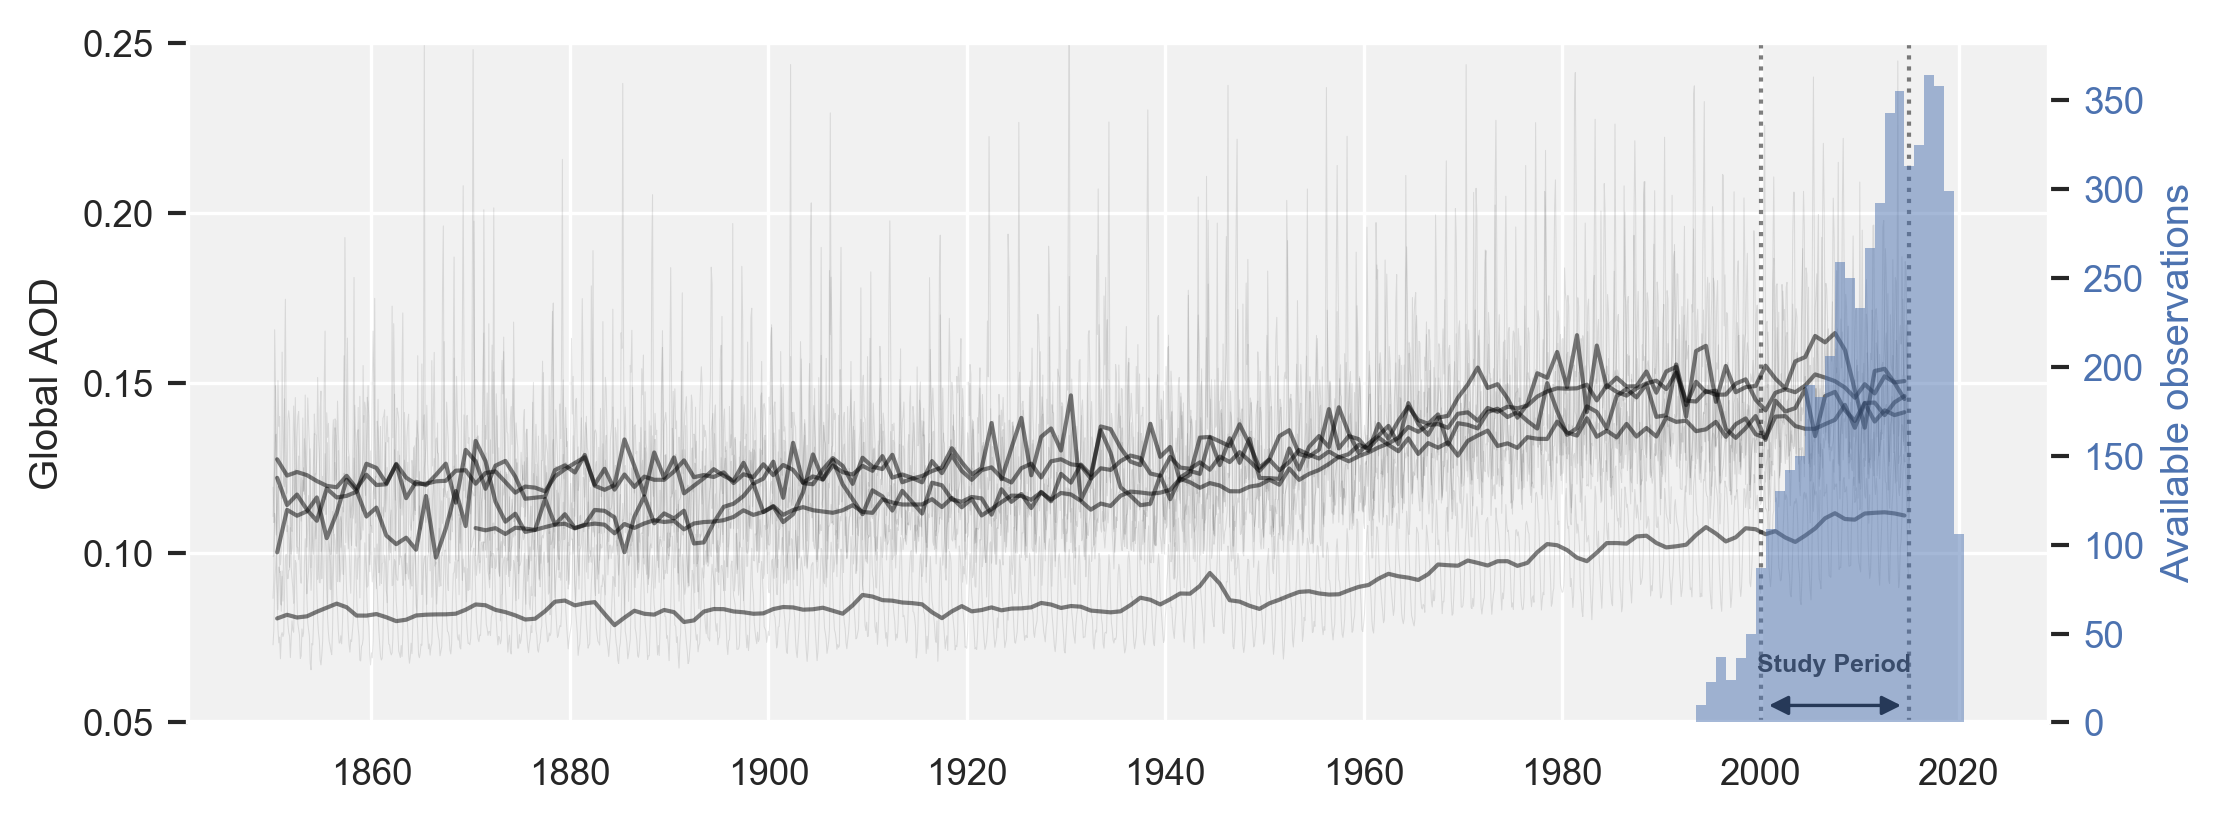
\includegraphics[width=12cm]{../scripts/figs/hist_runs.png}
 \caption{Global AOD computed from the model historical runs (OsloCTM3, GFDL-AM4, CanESM5, CESM2, IPSL-CM6A, ECHAM-HAM) and number of observation sites (AERONET).}
 \label{fig:hist_runs}
\end{figure}


\section{Datasets}
A set of nine column and in situ surface aerosol datasets are used in this study. The observation networks and the models providing output for these parameters are reported in Table \ref{table:datasets}.

\begin{table}
\footnotesize
 \begin{tabularx}{\textwidth}{lllX}
  \tophline
  Parameter   & Type    & Observation networks & Models                                                                                                    \\
  \middlehline
  AOD         & Column  & AERONET\textsuperscript{1}             & ECMWF-Rean; NorESM2; SPRINTARS; ECHAM-HAM; GEOS; OsloCTM3; GFDL-AM4; BCC-CUACE; CanESM5; CESM2; IPSL-CM6A \\
  AOD<1µm     & Column  & AERONET             & NorESM2; SPRINTARS; ECHAM-HAM; GEOS; GFDL-AM4                                                             \\
  AOD>1µm     & Column  & AERONET             & ECMWF-Rean; NorESM2; SPRINTARS; ECHAM-HAM; OsloCTM3; GFDL-AM4; BCC-CUACE                                  \\
  AE          & Column  & AERONET             & ECMWF-Rean; NorESM2; SPRINTARS; ECHAM-HAM; GEOS; OsloCTM3; GFDL-AM4                                       \\
  $PM_{2.5}$  & Surface & EMEP\textsuperscript{2}; IMPROVE\textsuperscript{3}                 & ECMWF-Rean;  NorESM2;  SPRINTARS;  ECHAM-HAM; GEOS                                                                                       \\
  $PM_{10}$   & Surface & EMEP; IMPROVE                 & ECMWF-Rean; NorESM2; SPRINTARS; ECHAM-HAM; GEOS                                                           \\
  $SO_{4}$    & Surface & EMEP; IMPROVE; CASTNET\textsuperscript{4}; CAPMoN\textsuperscript{5}; EANET\textsuperscript{6}             & ECMWF-Rean; NorESM2; SPRINTARS; ECHAM-HAM; GEOS; OsloCTM3; BCC-CUACE                                      \\
 $\sigma_{sp}$ & Surface & GAW-WDCA\textsuperscript{7}; IMPROVE; NOAA-FAN\textsuperscript{8}; ACTRIS; EMEP  & NorESM2                                                                                                   \\
  $\sigma_{ap}$  & Surface & GAW-WDCA; NOAA-FAN; ACTRIS; EMEP  & NorESM2; SPRINTARS                                                                                        \\
  \bottomhline
 \end{tabularx}
 \caption{List of observation and model datasets used in this study.
 \textsuperscript{1}Aerosol Robotic Network
 \textsuperscript{2}The European Monitoring and Evaluation Program
 \textsuperscript{3}Interagency Monitoring of Protected Visual Environments
 \textsuperscript{4}Clean Air Status and Trends Network
 \textsuperscript{5}The Canadian Air and Precipitation Monitoring Network
 \textsuperscript{6}Acid Deposition Network in East Asia
 \textsuperscript{7}Global Atmosphere Watch - World Data Centre for Aerosol
 \textsuperscript{8}National Oceanic and Atmospheric Administration Federated Aerosol Network
 }
 \label{table:datasets}
\end{table}

\subsection{Observations}

For each of the parameters used in this study, data of the highest quality level provided by the different observation networks were used. Mountain sites, corresponding to an elevation above 1000 m, were excluded for representativity reasons \citep{kinne2013mac}.

\subsubsection{AERONET Sun photometer}

The AErosol RObotic NETwork (AERONET) is a network established by NASA (National Aeronautics and Space Administration), and expanded by national and international collaborations. AERONET operates aerosol ground-based measurements in the different regions of the World \citep{holben2001emerging}. The observation of the columnar aerosols properties is performed by standardized and calibrated solar-powered CIMEL Electronique sunphotometers. These instruments measure the solar radiation reaching the surface of the Earth at different wavelengths and for different optical geometries. A new version of the sunphotometer (CE318-T) is also able to perform night-time measurements using the moon as light-source \citep{barreto2016new}. The direct measurements (aiming at the light-source) allow for the derivation of the Aerosol Optical Depth (AOD), and Angstrom Exponent (AE) which are related to the amount and size of the particles, respectively. The spectral information can be utilized to derive the AOD for the fine and the coarse particles, split by diameter less than or greater than 1 µm \citep{o2003spectral}. Three different data quality levels are available depending on the application of cloud filtering and correction for instruments calibration derivations \citep{smirnov2000cloud,smirnov2004aeronet}. The level 2.0 version 3 daily data, which provides automatic instrument anomaly quality controls \citep{giles2019advancements}, are used in this study for four different parameters:
AOD (calculated at 550 nm), AE (calculated using 440 nm and 870 nm channels), AOD<1µm, and AOD>1µm corresponding to the AOD of the particles whose diameter is lower and greater than 1 µm, respectively.

\subsubsection{Particulate Matter}
The particulate matter (PM) measurements are from EMEP (covering Europe), and IMPROVE (for North America). All the PM data have been made available via EBAS database infrastructure  (\url{http://ebas.nilu.no}), but the original IMPROVE data can be found in the VIEWS database (\url{http://views.cira.colostate.edu/}). Both $PM_{10}$ and $PM_{2.5}$ (\unit{µg.m^{-3}}) are used in this study.

The PM measurements in EMEP started around year 2000  \citep{torseth2012} and most of the sites use the gravimetric method for both size fractions, though some used automated monitors, i.e. a TEOM FDMS or b-attenuation. The EMEP monitoring complies with the European standards, i.e EN12341:2014 for the gravimetric methods and  EN16450:2017 for the automatic methods. 

The IMPROVE network has been operating since 1988 at remote and rural sites across the United States. IMPROVE uses four separate modules to collect samples for speciated $PM_{2.5}$ analysis and gravimetric $PM_{2.5}$ and $PM_{10}$ bulk mass measurements. Samples are collected every third day for 24 h and reported at local conditions. $PM_{2.5}$ and $PM_{10}$ mass concentrations are determined from Teflon filters from two separate modules sampling with $PM_{2.5}$ and $PM_{10}$ inlets, respectively. The gravimetric mass measurements are not performed at controlled relative humidity and temperature, and a laboratory relocation in 2011 resulted in unstable weighing conditions. Therefore, gravimetric mass measurements from 2011-2018 were subject to potentially high relative humidity conditions and likely contain particle bound water on the filters that could bias trends \citep{Hand2019}.



\subsubsection{$SO_{4}$ concentration}
 The global dataset is a subset of the data presented in \cite{aas2019global} and is based on data from different regional networks as described in Table \ref{table:datasets}.

The sulfate aerosol measurements are analysed from aerosol filters. In the EMEP,CASTNET, CAPMON and EANET networks these are either sampled with a $PM_{10}$ inlet or a no size cut off using a filterpack sampler  In the IMPROVE network sulfate measurements are done using a filterpack sampler with a $PM_{2.5}$ inlet. The filters are analysed to a large extend by ion chromatography after water extraction of the aerosol filter.

The data has been screened to be regionally representative and of satisfactory quality. Urban sites are not included, nor are sites where the surroundings have changed considerably in the period in question.
In \cite{aas2019global} the data  was averaged to monthly mean.  When the data have higher sampling frequency than daily, the sample is weighted in accordance with how many days it has been sampled in that month.

\subsubsection{Optical in situ}
Due to the scarcity of stations (only XXX), the presence of non-representative stations (e.g., stations located near roads), can have large effects on the computation of the regional time series. The urban stations have therefore been filtered out from this analysis. The level 2 data (quality controlled, hourly averaged, reported at STP) were used for two parameters measured by distinct instruments:

\begin{itemize}
 \item Scattering coefficient ($\sigma_{sp}$, in \unit{Mm^{-1}}), measured by integrating nephelometers. For bettery consistency in the models comparisons (model data is reported for RH=0\%), only the data with a relative humidity lower than 40\% were utilized \citep{pandolfi2018european}.
 \item Absorption coefficients ($\sigma_{ap}$, in \unit{Mm^{-1}}), from filter-based absorption photometers.
\end{itemize}

The same data selection (stations excluded, outlier removal, overlapping data) and correction (wavelength conversion) were applied as described in the companion AeroCom evaluation analysis \citep{jonaseval}.

\subsection{Models}
A set of 11 climate models are used in this study. Their main characteristics are reported in Table \ref{table:models}. These models can be separated into three main groups.

\subsubsection{CAMS-Reanalysis}
The CAMS reanalysis, which is the successor to the MACC reanalysis (Monitoring Atmospheric Composition and Climate), is the latest global reanalysis dataset of atmospheric composition produced by the Copernicus Atmosphere Monitoring Service \citep{inness2019cams}. It is produced using 4DVar data assimilation in the CY42R1 model cycle of the ECMWF (European Centre for Medium-Range Weather Forecasts) Integrated Forecast System (IFS), with 60 hybrid sigma/pressure vertical levels. The model used in the CAMS reanalysis includes several updates to the aerosol and chemistry modules on top of the standard CY42R1 release. The IFS model assimilates several satellite products, from aerosols (AOD) to greenhouse gases (CO2, CH4) \cite{inness2019cams}.

The daily data, from the ECMWF data archive (MARS), were used in this study. The CAMS reanalysis dataset covers the period January 2003 to near real time. The three first years of the trends study period (2000-2002) are missing for this model.

\subsubsection{AeroCom phase III}
The AeroCOM-project is an open international initiative of scientists interested in the advancement of the understanding of the global aerosol and its impact on climate \citep{schulz2006radiative}. Different model experiments have been conducted during the third phase of this project, initiated in 2015, in order to investigate specific topics (dust, volcanic aerosols, aerosol absorption, ...). 

In this study, we use the model outputs from the historical experiment, whose main aim is to understand the regional trends in aerosol distribution from 1850 to 2015 and to quantify the aerosol forcing with a main emphasis on the direct aerosol effect. The models can be run in various configurations: fixed sea-surface temperature (SST), historically evolving SSTs or fixed meteorology for one year. 

\subsubsection{CMIP6}
The upcoming 2024 IPCC sixth assessment report (AR6) will feature new state-of-the-art CMIP6 (Couple Model Intercomparison Project, Phase 6) models with model runs in higher resolution and with new physical processes. An overview of the experimental design and organisation can be found in \cite{eyring2016overview}. 

In this study, we use the data of four CMIP6 models from the historical experiment, which provide output from 1850 to 2014, selected as the last year of the study period of this analysis.

\begin{table}[]
\footnotesize
 \begin{tabularx}{\textwidth}{llllllX}
  \toprule
  Model      & Group     & \begin{tabular}[c]{@{}l@{}}Natural \\ interactive emissions\end{tabular} & \begin{tabular}[c]{@{}l@{}}Anthropogenic \\ emissions\end{tabular} & Meteorology & \begin{tabular}[c]{@{}l@{}}Res \\ (degree)\end{tabular} & References                                                          \\ \midrule
  ECMWF-Rean & CAMS-Rean & D, SS                      & MACCity & RA & 0.7x0.7                  & \cite{inness2019cams,zhang2009asian}                                                                    \\
  SPRINTARS  & AP3       & D, SS, DMS, Oc VOC      & $SO_{2}$, BC, OC                & N           & 0.56x0.56                  & \cite{takemura2000global,takemura2002single,takemura2005simulation} \\
  ECHAM-HAM  & AP3       & D, SS, DMS                          & $SO_{2}$, BC, OC                          & fSST           & 1.875x1.875                  &  \cite{tegen2019global,neubauer2019global}                                       \\
  GEOS       & AP3       & ?                          & ?                          & ?           & 1.00x1.00                  &           ?                                                          \\
  OsloCTM3   & AP3       & ?                          & ?                          & ?           & 2.25x2.25                  & \cite{lund2018concentrations,myhre2009modelled}                     \\
  GFDL-AM4   & AP3 & D, SS, DMS, Oc\&Veg OC, & \chem{SO_2}, \chem{SO_4}, BC, OC & fSST\&N  & 1.x1.25 &  \cite{zhao2018agfdl,zhao2018bgfdl}                 \\
  BCC-CUACE  & AP3       & D, SS, DMS                          & $SO_{2}$, BC, OC                         & F           & 2.8x2.8                  & \cite{zhang2012simulation,zhang2014application,wang2014improvement}                                                                    \\
  NorESM2    & CMIP6     & D, SS, DMS, MSA, BVOC      & C                          & F           & 1.89x2.50                  & \cite{olivieprep, selandprep, kirkevag2018production}               \\
  CanESM5    & CMIP6     & ?                          &             ?               & ?           & 2.77x2.81                  & \cite{gmd-12-4823-2019}                                             \\
  CESM2      & CMIP6     & ?                          & ?                          & ?           & 0.94x1.25                  &             ?                                                        \\
  IPSL-CM6A  & CMIP6     & ?                          & ?                          & ?           & 1.27x2.50                  &              ?                                                       \\ \bottomrule
 \end{tabularx}
 \caption{Information on models used in this study.
  Anthropogenic emissions (C=CMIP6-CEDS, O=other, *=CMIP6 modified)
  Interactive natural emissions (D=dust, SS=sea salt, O=biogenic organic, V=volcanic, Oc=Oceanic, Veg=Vegetation)
  Meteorology (N=nudged to analysed meteorology, S=prescribed varying meteorology, G=coupled GCM, F=Free, fSST=fixed SST/SIC monthly fields, not nudged, RA=combined reanalysis of meteorology and composition)
 }
 \label{table:models}
\end{table}

\section{Methods}

\subsection{Regional time series}
Due to the nature of the processes involved in the emission and the deposition of aerosols, one can expect different trends in different regions of the World. Instead of combining the trends obtained at each individual observation station in a given region, regional time series are computed by assembling directly the measurements of these stations. A first advantage of this method is that a single trend can be computed in a given region, with an associated significance and uncertainty, which it is not possible to get when combining the trends for individual sites together together. Also, even when a station has not provided a sufficient amount of data for computing the trend at its location, the data can still contribute to the computation of the regional time series. The computation of regional time series should be performed in regions exhibiting similar seasonal patterns, which constrains the maximum size of the regions.

\subsubsection{Regions definition and observations coverage}
Seven regions are considered in this study. The definition of these regions enables restriction of the study to a limited number of geographic areas, but also provides a global coverage when considering the ensemble of those regions. As seen in Figure \ref{fig:map_obs}, the regions do not have a similar coverage in terms of observations. North America and Europe have the highest concentrations of instruments.
\begin{itemize}
 \item AERONET is the most important network in terms of number of instruments. More than 1000 observation points, with more or less long time series, are found across the globe. The highest density of instruments is in Europe and in the central part of North America (US). The lowest densities are found in southern Africa and Australia.
 \item Particulate Matter: 212 instruments are spread mostly over Europe and North America. 
 \item $SO_{4}$: 346 instruments are operating, mostly in North America and Europe. A few stations are also located in Asia and North Africa.
 \item $\sigma_{sp}$ and $\sigma_{ap}$: about 50 stations are spread over North America, Europe, North Africa and Asia. Due to time coverage issues, the data up to the year 2018 were used to compute the regional time series of these two parameters.
\end{itemize}

In order to assemble the sites most affected by Saharan dust, the North Africa region has been extended in the North beyond the continent border. Stations located in the South of Spain, Cyprus and Greece contribute to the regional time series in the region we are calling North Africa.

\begin{figure}
 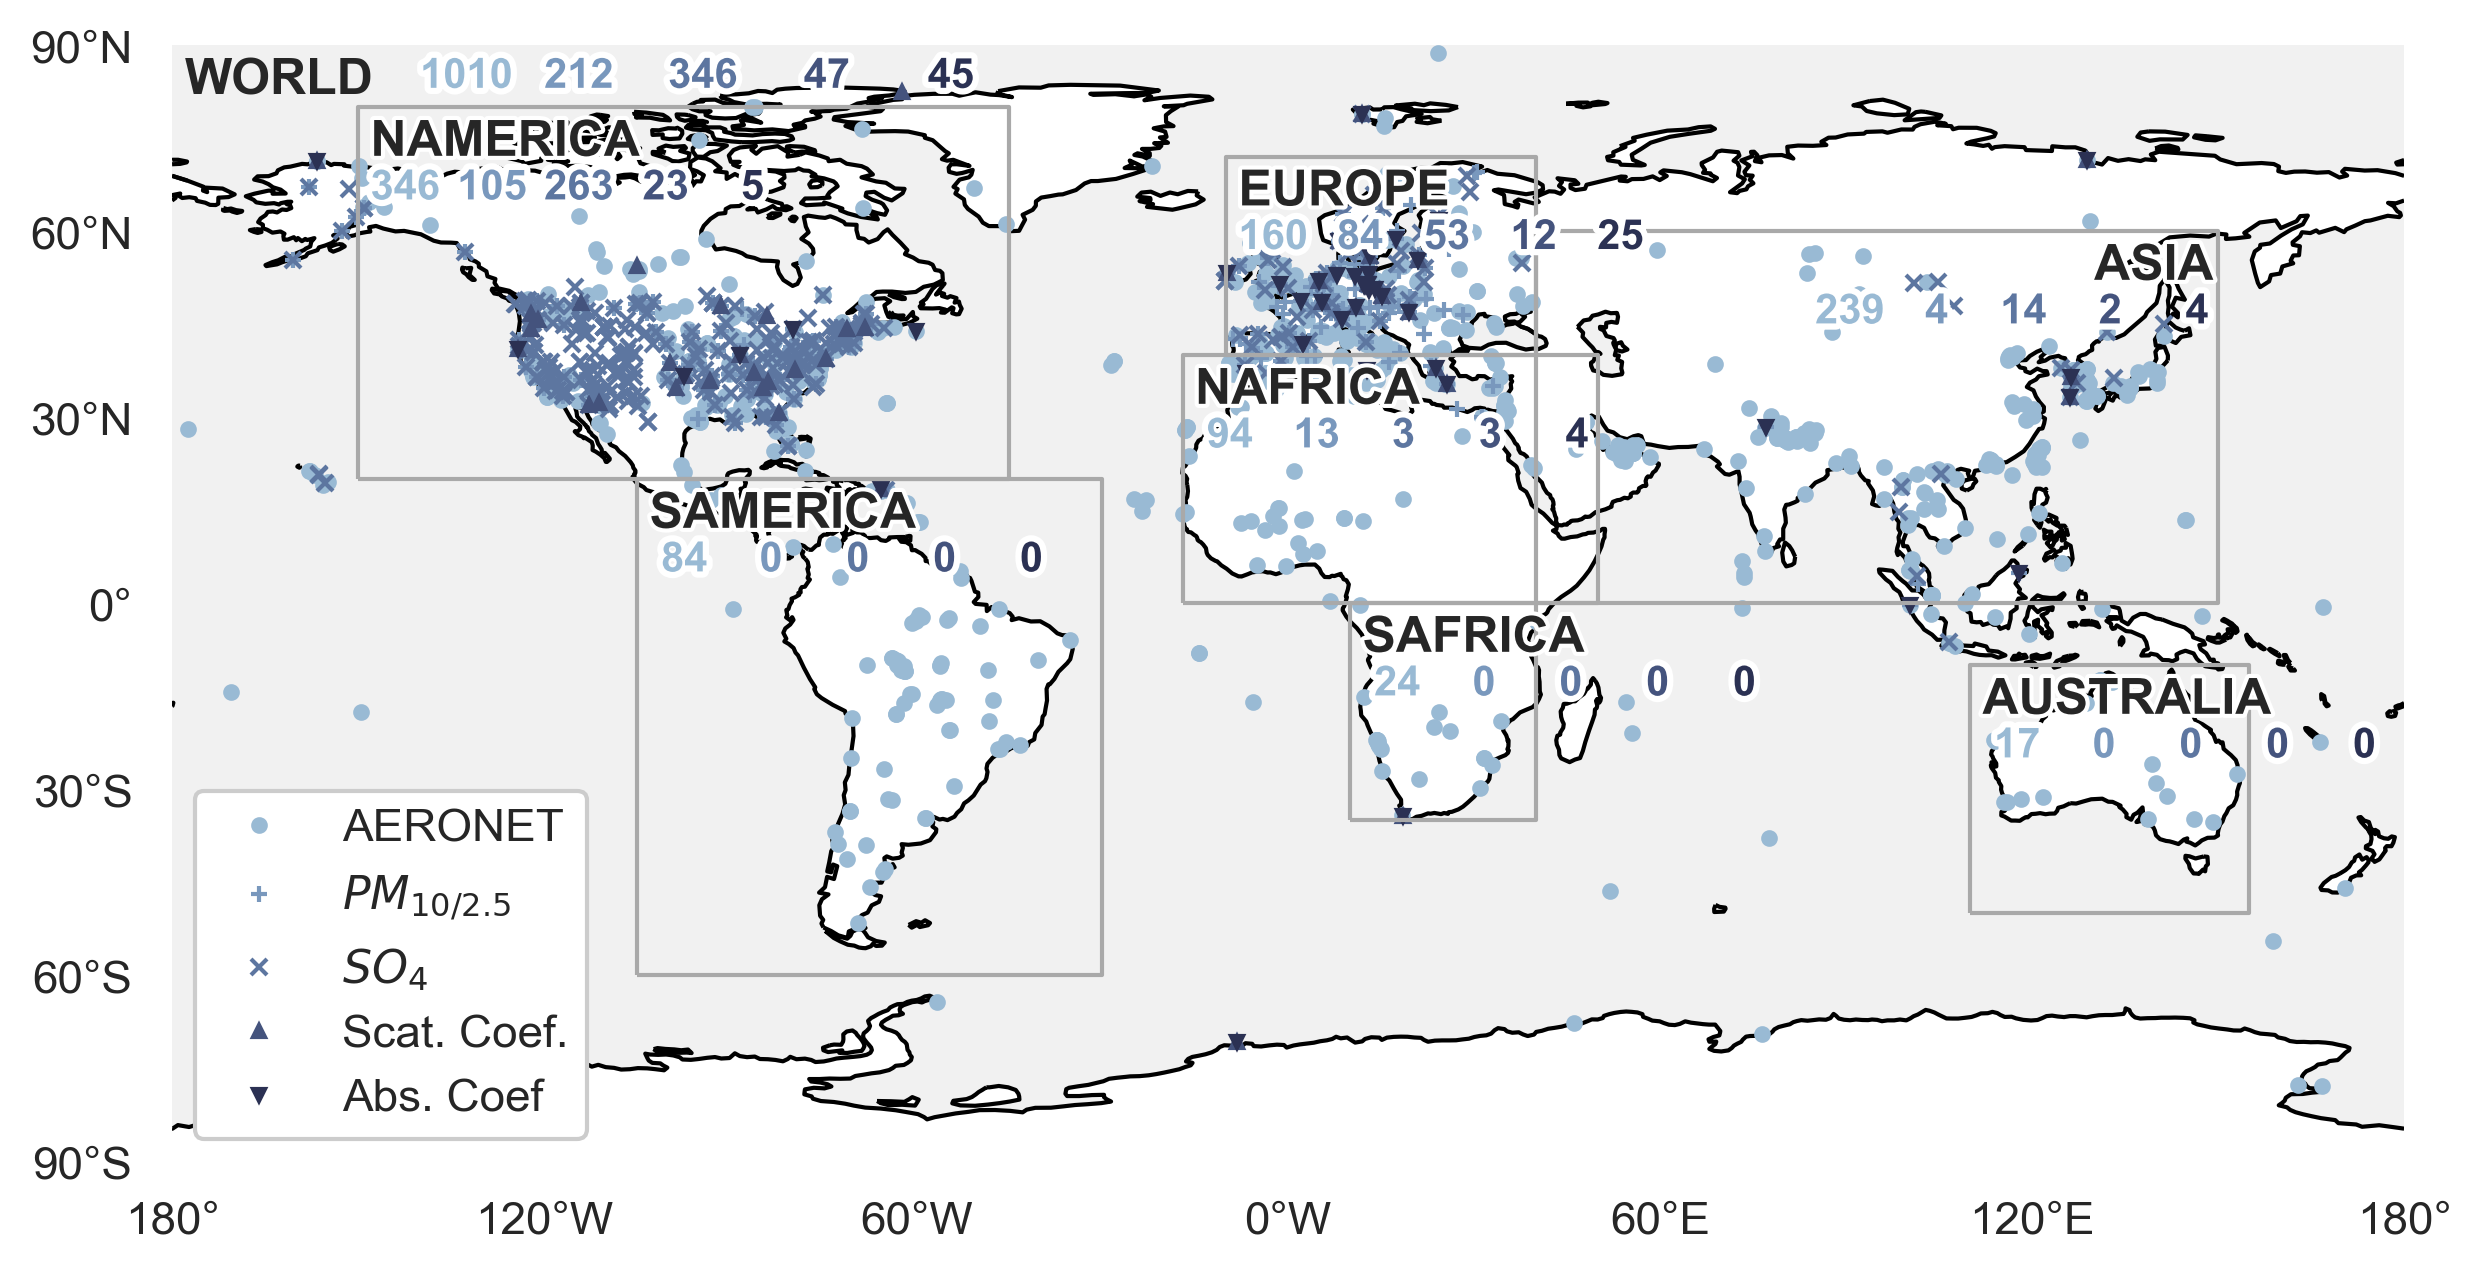
\includegraphics[width=12cm]{../scripts/figs/maps/av_obs.png}
 \caption{Distribution of the observations within the different regions considered in this study. The numbers reported within each region correspond to the maximum number of stations given for each observation network.}
 \label{fig:map_obs}
\end{figure}

\subsubsection{Time constraints}
The regional time series are computed by combining, for each timestamp, the valid data of all the stations in the corresponding region. In order to construct consistent and robust regional time series, some additional data constraints are required to provide a valid point (a station with valid measurements) in the regional time series. Very short term stations (e.g AERONET DRAGON stations) are eliminated by requiring a minimum of 300 valid daily measurements, which reduces, as an illustration, the number of AERONET stations from 1010 to 437. A minimum of three valid points (daily or monthly depending on the available resolution) is required per timestamp for the calculation of the regional time series in this timestamp. The list of the station names contributing to the computation of the regional time series can be found in supplementary.

\begin{figure}
 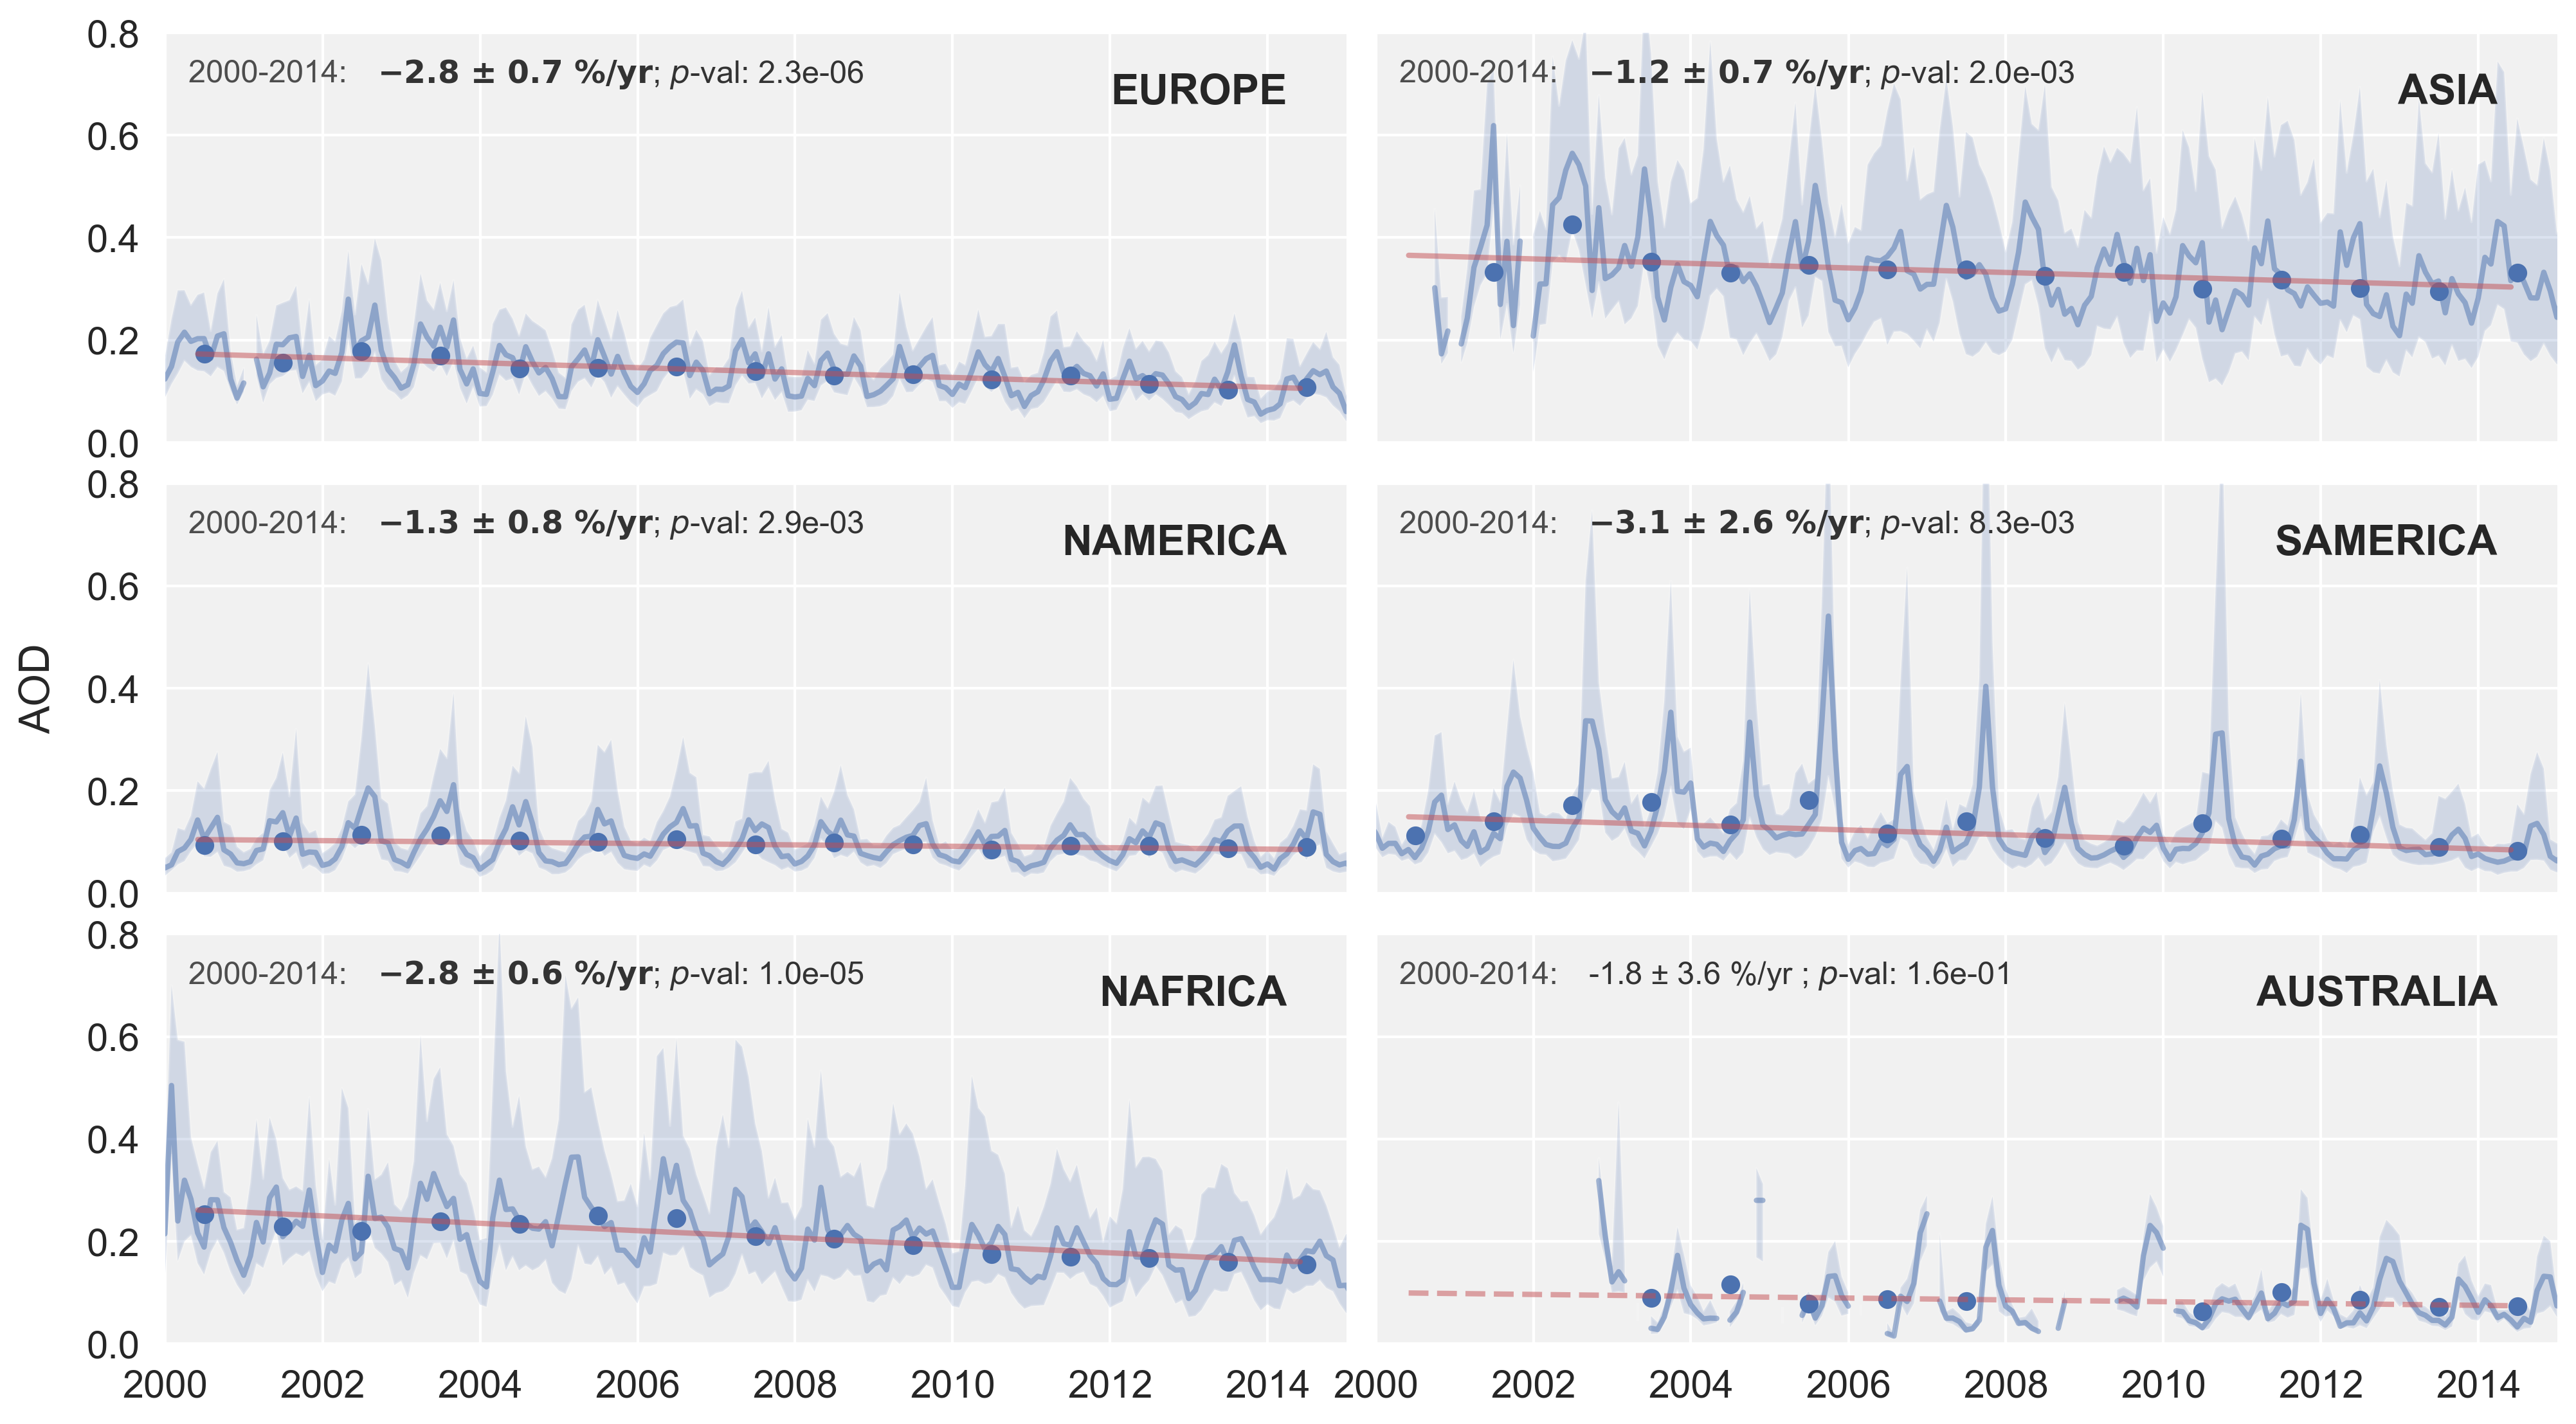
\includegraphics[width=16cm]{../scripts/figs/ts/panel-od550aer.png}
 \caption{Regional time series of AOD. The dark blue line and the light blue envelope correspond to the median and the first and third quartiles of all the valid points at the corresponding timestamp, respectively. The blue dots correspond to the yearly averages which are used to compute the linear trend, displayed as a continuous line when the trend is significant and a dashed line when it is not.}
 \label{fig:ts_aod}
\end{figure}

When those criteria are fulfilled, the median, the first and third quartiles are computed at the finest time-resolution available. The quartiles provide an indication of the inter-regional variability. An example of a regional time-series is shown in Figure \ref{fig:ts_aod} for AOD.


\subsection{Trends calculation}

\subsubsection{Regional time series computation}
The trends are computed based on the yearly averages of the regional time series. Using the yearly averages eliminates any issues caused by the seasonal cycles (observed for most of the aerosol parameters used in this study) during the calculation of the trend slope. In order to insure the statistical robustness of these yearly averages, the time averaging is performed step-by-step with specific time constraints. By starting at the finest time resolution available in the data, monthly, seasonal and yearly averages are computed when the following criteria are fulfilled:
\begin{itemize}
 \item at least 5 days per month (when daily observations are available).
 \item at least 1 month per season.
 \item 4 seasons per year.
\end{itemize}
These temporal constraints offer a reasonable compromise between the availability and the robustness of the yearly statistics.

\subsubsection{Trends computation}
The same methodology as described by \cite{aas2019global} was used to derive the trends of the regional time series. The significance of the trends is tested with the Mann-Kendall test. The related p-value is used to determine if the trend is significant or not within a confidence interval of 95\%. The slope is calculated with the Theil-Sen estimator which is less sensitive to outliers than standard least-squares methods. At least least 7 valid yearly averages (50\% of time coverage) are required in the regional time series for the computation of the slope.

An uncertainty is provided for each trend by combining the error of the slope calculation itself to the error of the residuals:

\begin{equation}
 Uncertainty = \sqrt{{\left (\frac{\Delta m}{y(2000)}\right )}^{2} + {\left ( \frac{m \cdot \Delta r}{y(2000)^2}\right )}^{2} }
\end{equation}

where $\Delta m$ is the Theil-Sen estimator 95\% confidence interval, $y(2000)$ is the value of the regression line at the year 2000, $m$ is the value of the Theil-Sen slope and $\Delta r$ is the averaged error on the residuals.

The trend is provided as a relative trend (\%/yr) with respect to the first year of the time period (2000).

\subsection{Representativity of the trends}
The number of available points used to compute the regional time series is not constant in time. For a given observation station, the number of points available might vary in time due to the nature of the measurements. For instance, classic sun photometers only measure in the daytime. Due to seasonal daylight and cloud condition variations, clear seasonal cycles are observed in the number of observations of AOD. The density of the different observation networks can also change with time. The early development of the different observation networks usually coincided with an increase in the number of observation stations. More recently, primarily for funding reasons, some networks have reduced the number of stations. This variation in the number of available measurements raises the question of time representativity for the computation of the trends.

Associated with this time representativity issue comes the space representativity issue. The data coverage is uneven across the different regions. Moreover, within a single region, the observation stations might be located in contrasting environments. Stations located in environments that are more urban, or rural, or mostly affected by natural particles, might have trends differing from the trend associated with the whole region.

Some studies have focused on the representativity of the observation stations by investigating the biases of different optical properties \citep{wang2017,schutgens2017spatio,schutgens2019site}. This analysis is dedicated to the  representativity of the observation networks specifically for the computation of the trends. These two issues might give different results, since a stations associated with a bias, could still have a representative tendency. In order to evaluate the effect of the partial space and time sampling of the observations for the evaluation of the trends, two sensitivity studies, focusing on the time sampling and the space sampling, have been conducted using model subsets of data. For each of these studies, the trends are computed for one reference ($Ref$) and one experiment ($Exp$) dataset, and compared with each other.
\begin{itemize}
 \item Time representativity study
       \begin{itemize}
        \item $Ref_{time}$: Collocation in space and time
        \item $Exp_{time}$: Collocation in space using complete time-series
       \end{itemize}
 \item Space representativity study
       \begin{itemize}
        \item $Ref_{space}$: Collocation in space using complete time-series (=$Exp_{time}$)
        \item $Exp_{space}$: All grid-points in region using full time-series
       \end{itemize}
\end{itemize}

The difference between the relative trends are computed for each parameter and region. Those differences are then converted into a score (\unit{\%}) by using a normal distribution $f$ described by a mean $\mu=0$ and a standard deviation of $\sigma=0.5$. The choice of these parameters leads to a representativity score of 100\% when there is no difference in the trends of a reference and an experiment dataset, while a difference of 0.5\%/yr would indicates a representativity score of 50\%.

For a given parameter $p$ and a region $r$, the Representativity $Rep(p,r)$ is calculated as following

\begin{equation}
 Rep_{space,time}(p, r) = {f\left(\left| \tilde{t}_{Exp_{space,time}(p, r)}-\tilde{t}_{Ref_{space,time}(p, r)} \right|\right)}
\end{equation}
where $\tilde{t}$ is the relative trend of the corresponding dataset.

Finally, the total score is computed as the mean of the time and the space representativities. This parameter provides a

\begin{figure}[t]
 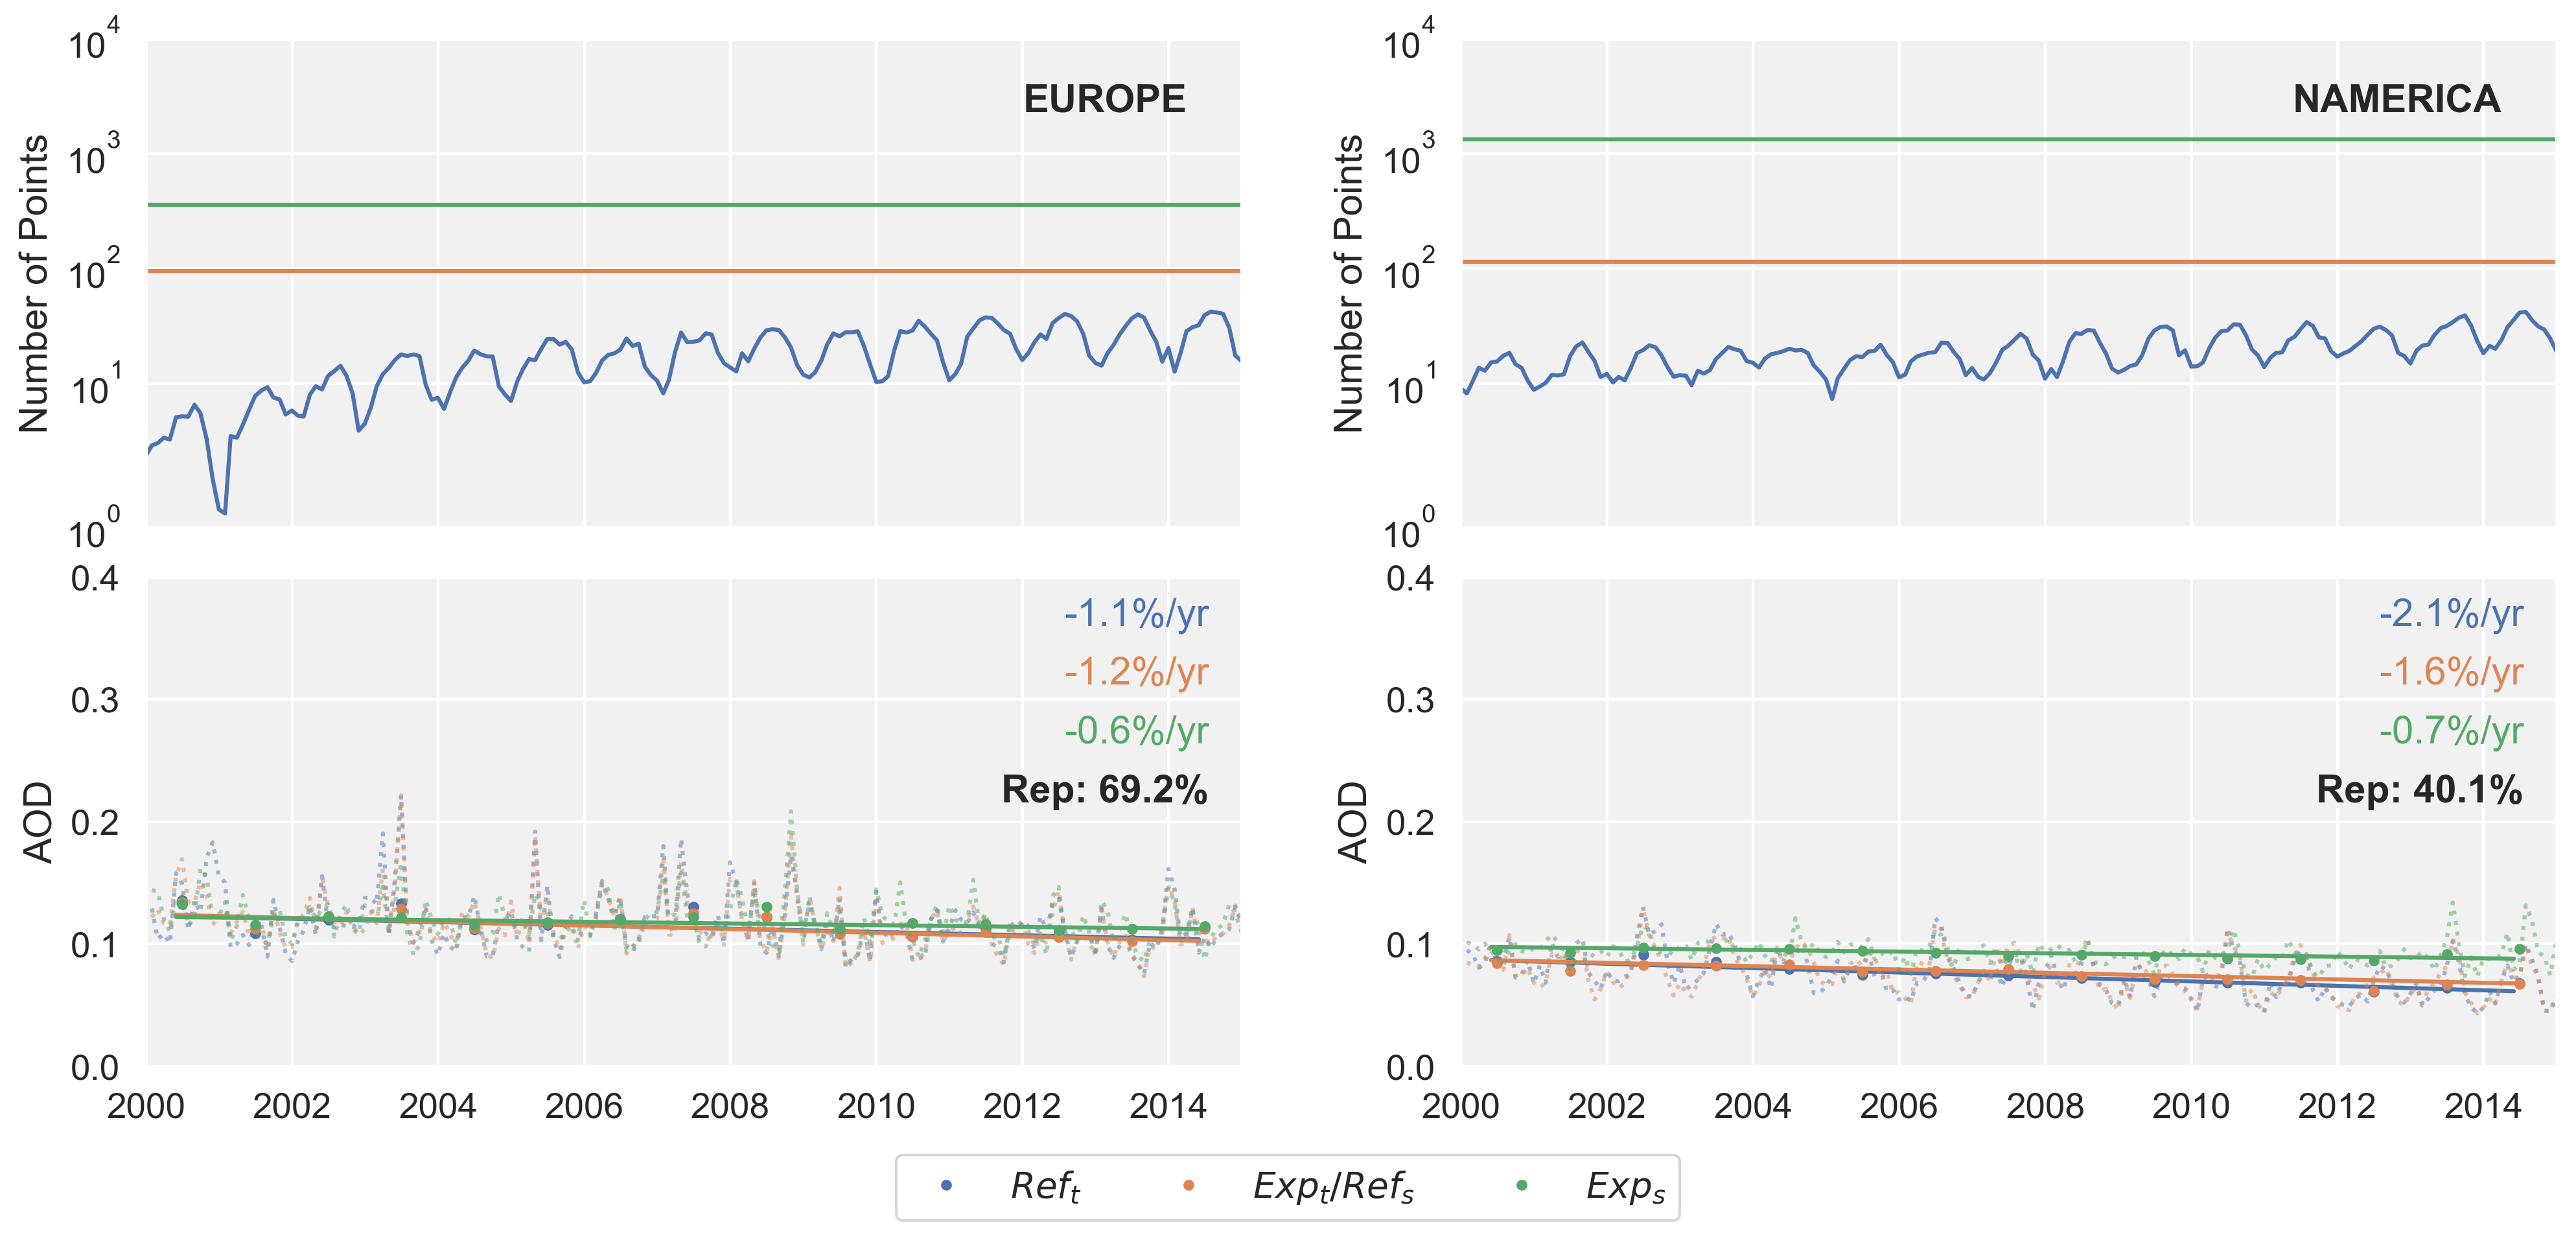
\includegraphics[width=16cm]{../scripts/figs/representativity-od550aer.png}
 \caption{Representativity of the regional AOD time series for the computation of trends assessed with model data. The upper figures correspond to the number of points used to compute the regional time series for the three different datasets. The lower figures show the time series, the trends, and the resulting representativity. $Ref_{time}$ corresponds to the model output collocated in space and time to the available observations. $Exp_{time}/Ref_{space}$ corresponds to the model output collocated in space to the stations providing measurements, using complete time series from 2000 to 2014. $Exp_{space}$ corresponds to the model output in the region without any collocation to the observations (using all gridpoints in the region).}
 \label{fig:representativity}
\end{figure}

An example of the calculation is presented in \ref{fig:representativity} for AOD in Europe and North America. In both regions, the $Ref_{time}$ dataset, corresponding to the available observations, reveals strong seasonal cycles when considering the number of points used to compute the regional time-series. These cycles are observed with most of the sun photometer datasets since the instruments only operate during daytime and cloud free conditions, and the amount of daylight and clouds varies with the season. Together with this seasonal cycle, one observes an increase in the number of points with time, which reflects the increasing number of stations over these two regions. The trends in Europe shows similar values for the time study, which means that the trend is not greatly affected by the variation of the available measurements in time. The difference is larger when considering all the grid-boxes of the domain, but the overall difference of the two studies corresponds to a representativity of 69\%. In North America, the differences in the trends between the different data sets are larger, especially for the space study. This means that the trend obtained in the whole region is significantly different from the trend obtained when considering only the grid points where observation stations are located. It should however be mentioned that the ocean grid-points are not filtered out when computing the trends over the whole domain. For this reason, the regions containing a greater proportion of ocean grid-points, where the trends are most likely to differ from those observed over land, will tend to have a lower spatial representativity.

This representativity study illustrates that the partial coverage in time and space of the observations leads, in some cases, to artificial trends. The representativity scores are discussed for each parameter in the following section together with the trends results.

\section{Results}

\subsection{Trends in observations}\label{obs_trends}
This sections presents the trends in the observations computed for the different parameters and over the predefined regions.

\begin{table}
 \begin{tabular}{lllllll}
  \tophline
                     & EUROPE & NAMERICA & SAMERICA & NAFRICA & ASIA & AUSTRALIA \\
  \middlehline
  AOD                & 0.17   & 0.10     & 0.15     & 0.26    & 0.35 & 0.10      \\
  AOD<1µm            & 0.14   & 0.08     & 0.12     & 0.11    & 0.18 & 0.05      \\
  AOD>1µm            & 0.03   & 0.02     & 0.03     & 0.10    & 0.11 & 0.03      \\
  AE                 & 1.44   & 1.46     & 1.30     & 0.72    & 1.06 & 0.97      \\
  $PM_{2.5}$ (\unit{µg.m^{-3}})     & 12.8   & 7.3      & -        & -       & -    & -         \\
  $PM_{10}$ (\unit{µg.m^{-3}})      & 16.8   & 12.8     & -        & 19.6    & -    & -         \\
  $SO_{4}$ (\unit{µg.m^{-3}})       & 2.01   & 1.45     & -        & 2.98    & 1.97 & -         \\
  $\sigma_{sp}$ (\unit{Mm^{-1}}) & 33.2   & 25.0     & -        & -       & -    & -         \\
  $\sigma_{ap}$ (\unit{Mm^{-1}})  & 9.7    & 2.7      & -        & -       & -    & -         \\
  \bottomhline
 \end{tabular}

 \caption{Observations means for the year 2000 (reference year used for computing the relative trends). Each value is extracted as the intercept of the linear trend computed in the 2000-2014 period for all the parameters, except for for $\sigma_{sp}$ and $\sigma_{ap}$ for which the trends have been computed over 2000-2018 for time coverage reasons. One could mention that with the minimum number of yearly averages set to seven, no trend could be processed in the southern Africa region.}
 \label{table:obs_2000mean}
\end{table}

In order to compare the trends observed for the set of nine aerosol parameters in a consistent manner, we focus on the relative trends, with the reference set to the year 2000, as the first year of the study period. The means for the year 2000, reported in Table \ref{table:obs_2000mean}, reveal a great inter-regional variability.

The AOD is more than three times higher in Asia (AOD=0.35) than in North America and Australia (AOD=0.10). Intermediate AOD values are found in Europe and South Africa, while the second highest load is found in North Africa (AOD=0.26). In most regions, the AOD is largely dominated by its fine fraction (AOD<1µm), but this is not the case in North Africa (or Australia), where the persistent presence of desert dust makes the coarse mode (AOD>1µm) contribution to the total AOD similar in size to the fine mode contribution. This predominance of coarse particles is reflected in the AE values which exhibit lower values in North Africa (AE=0.72) and Australia (AE=0.97).

The PM observations are primarily available from Europe and North America. $PM_{10}$ observations are also available in the North Africa region as defined in this analysis, but these stations are  located in the northern part of the region, in other words in southern Europe, which is less affected by the dust sources than the AERONET stations, which covers the whole region including located in surrounding deserts. Both $PM_{10}$ and $PM_{2.5}$ are larger in Europe than in North America, with different relative proportions. In Europe, $PM_{2.5}$ represent 75\% of the $PM_{10}$, as compared to on 57\% in North America.

$SO_{4}$ means (surface mass concentrations) for the year 2000 ranges between 1.45 and 2.98 \unit{µg.m^{-3}} with the low value occurring in North America and the high value for North Africa (southern Europe). Similar means are found in Europe and Asia, around 2 \unit{µg.m^{-3}}, though one should bare in mind that there are relatively few sites in Asia and they are not located in the most polluted areas in China and India \citep{aas2019global}.

Analogous to the surface $PM_{10}$ measurements, $\sigma_{sp}$ is higher in Europe (33.2 \unit{µg.m^{-3}}) than in North America (25.0 \unit{µg.m^{-3}}). The same feature is found for $\sigma_{ap}$ which also has higher values in Europe.

\begin{figure}[t]
 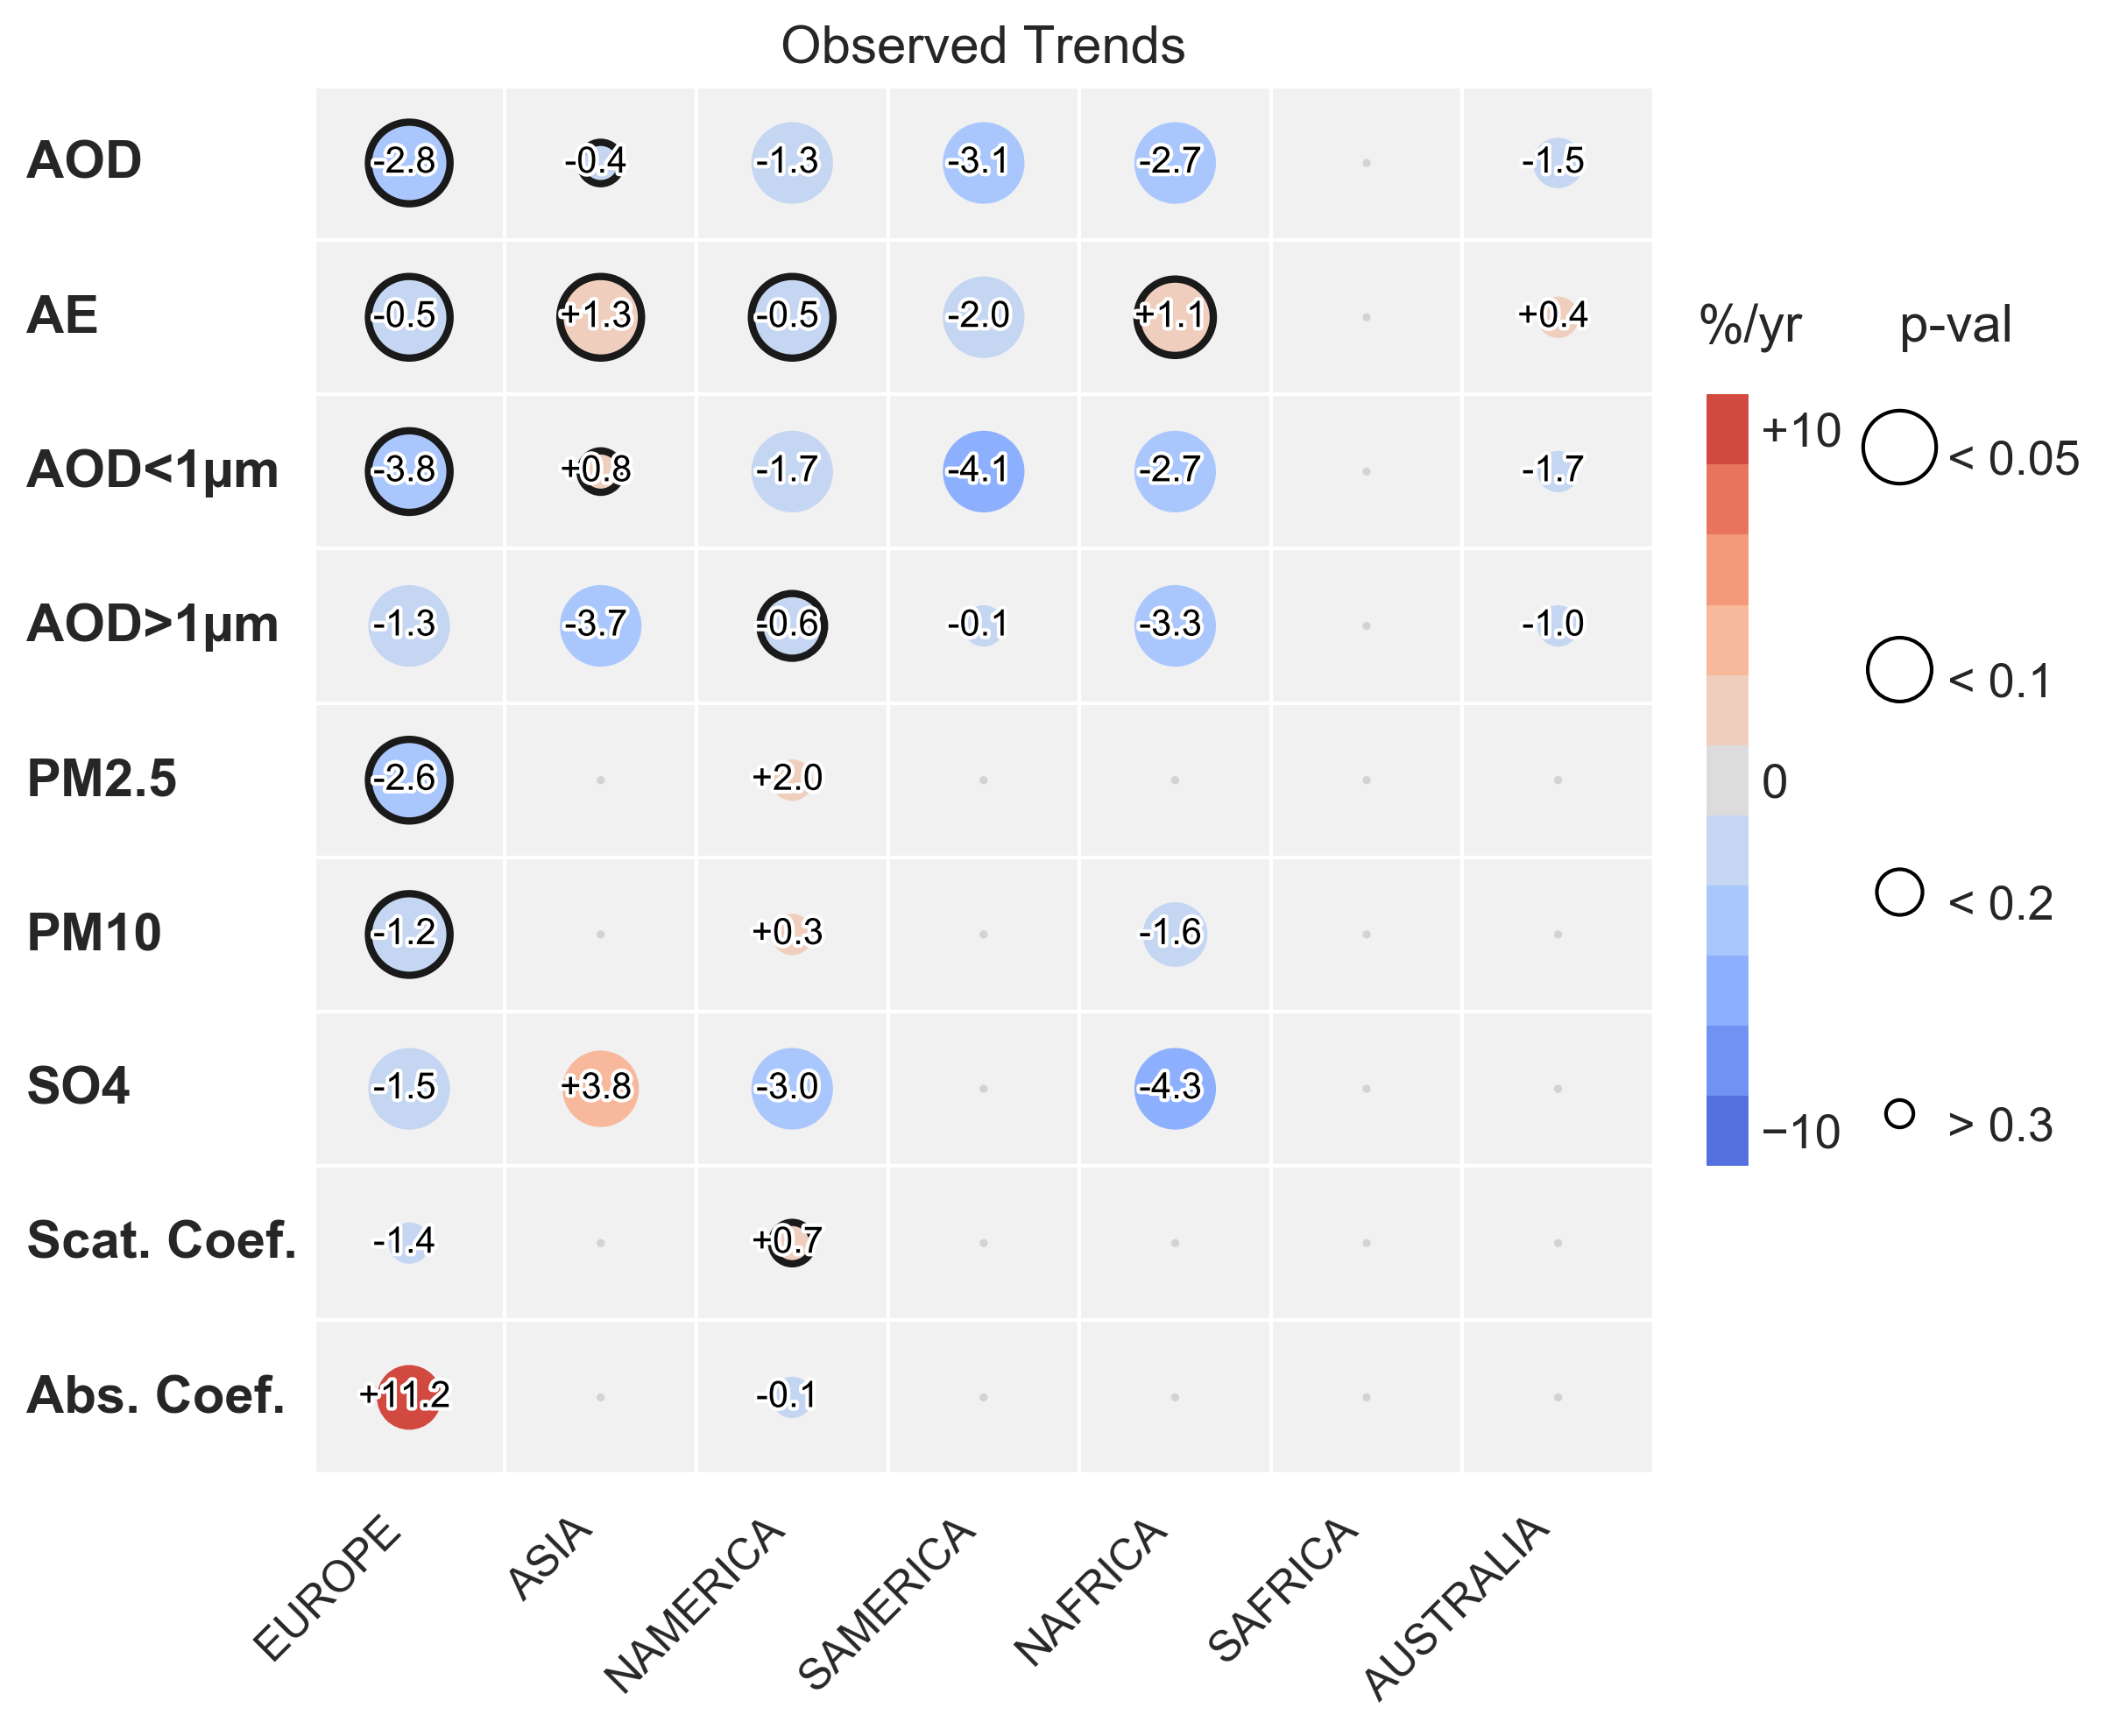
\includegraphics[width=12cm]{../scripts/figs/heatmaps/OBS.png}
 \caption{Regional trends of the aerosol properties computed with the observation datasets. The color of the circles corresponds to the slope, while the radius indicates the p-value. The largest circles represent the trends significant with a confidence of 95\%. The circles bordered with a black line indicate the trends associated with a representativity greater than 50\%.}
 \label{fig:obs_trends}
\end{figure}

The relative trends for the 2000-2014 period are shown in Figure \ref{fig:obs_trends}. The heatmap is dominated by the blue color, which indicates mostly negative trends, especially when considering the extensive parameters. Usually, the lowest p-values (<0.05) are associated with the lowest uncertainties. Each of the largest circles are then associated with a certain decrease/increase since the value of the trend is greater than the uncertainty. The uncertainties are presented in Figure \ref{fig:bars}.

\begin{itemize}
 \item In Europe, both columnar and surface parameters reveal significant decreases, with the exception of $\sigma_{ap}$ for which the observed decrease is not significant. For this last parameter, the associated uncertainty of the trend exceeds the trend itself. This large uncertainty is induced by the low data coverage in the earliest period. For the other parameters, the uncertainties are lower than the trends. A decrease in AOD (-2.8\%/yr) is found for both fine and coarse mode particles. This is consistent with the negative trends found at some individual stations in this region \citep{glantz2019}. The fine mode is decreasing more than the coarse mode, which is consistent with the decrease observed for AE. The same pattern is found at the surface since $PM_{2.5}$ has decreased by factor of two relative to $PM_{10}$. These trends could result from the mitigation measures aiming for reduced anthropogenic aerosols emissions. This is more directly observed in the decrease of $SO_{4}$ (-1.5\%/yr). This is somewhat lower trend than what was reported in \cite{aas2019global} (-2.67\%/yr), but this is due to the selection of region areas. The sites in Northern Africa which do show more reductions (-4.3\%/yr) are part of the European continent. 
 
 The representativity study reveals that the observed trends are actually representative for the whole period and region for all of the parameters, except for $\sigma_{sp}$ and $\sigma_{ap}$ due to the lack of observations in the earliest period. A good agreement is found with the trends obtained at individual stations and reported by \cite{collaudcoenprep}, which reports on decreases of -2.92\%/yr for $\sigma_{sp}$ and -4.2\%/yr for $\sigma_{ap}$, as compared to -2.5\%/yr and -2.0\%/yr in this study.
 \item In North America, similar trends are found for the columnar properties as were found for Europe. AOD is decreasing at a rate of 1.3\%/yr, a 55\% percent smaller trend than observed in Europe, but the North America reference value in 2000 is 40\% lower than the reference value in Europe. The decreases observed for both $PM_{2.5}$ (-2.1\%/yr) and $PM_{10}$ -1.6\%/yr are significant and in the same range of values than the trends found in Europe. However, the actual trends are probably somewhat higher than found here. The possible bias is caused by increased relative humidity during weighing, thus more particle bound water, after the relocation of the laboratory in 2011. \cite{Hand2019} reported that the  decrease in $PM_{2.5}$ from 2005 through 2016 was -2.6\%/yr, while it was -3.9\%/yr for the reconstructed fine mass correcting for the possible bias in the measurements. $SO_{4}$ decreases by about 3\%/yr, which is twice as large as the decrease observed in Europe, where the reference value is however larger than in North America. The sulfate trend is similar to the trend reported by \cite{aas2019global} in this region (-3.15\%/yr). The regional time series are extend farther back in time for $\sigma_{sp}$ and $\sigma_{ap}$ in North America than in Europe. However, no significant trends are found for these data sets. One can note that the representativity scores are higher for AE than for AOD, while these two parameters have the same amount of data. This means that the trends are probably smoother, in space and time, when comparing AE with AOD, which makes a same amount of available observations more representative in the first case. \cite{collaudcoenprep} finds a large decrease for $\sigma_{sp}$ (-2.57\%/yr) which is not found in this study, when using regional averaged time series to calculate the trend rather than regionally averaged trends. Similar values are found in this study and by \cite{collaudcoenprep} for $\sigma_{ap}$ (-1.85\%/yr) despite the fact the trend is not significant. The IMPROVE network also measures filter absorption using a Hybrid Integrating Plate and Sphere (HIPS) system \citep{Warren2016}. These data are not included in this study, but \cite{Warren2016} reports a significant decrease (-2.7\%/y) in the light absorption coefficients from 2005 to 2015.
 \item All of the columnar properties show decreasing trends in South America. All the trends are significant, except for AOD>1µm. As shown in the regional time series in Figure~\ref{fig:ts_aod}, the observed decrease in AOD coincides with a global diminution of the intensity of the seasonal peaks happening around September and resulting from the Amazonian forest fires \citep{aragao201821st}. These peaks are highly variable from year to year and could greatly affect the trend when considering another time period. With a rate of -2.0\%/yr, the largest decrease of AE is found in this region. While no significant trend is found for AOD>1µm, the tendency to increasing coarse particles is probably due to the production of local dust as a result of the increasing deforestation \citep{werth2002local,betts2008effects}.
 \item In North Africa, while significant decreases are found for all AOD parameters, an increase of AE (+1.1\%/yr) is observed, which indicates an increase in the proportion of fine particles with time. This is consistent when considering the AOD of the fine and coarse modes, which reveal a larger decrease for AOD>1µm. \cite{chin2014multi} also found a decrease in dust in the Sahara/Sahel in the time period 1980-2009 due to reduced 10m-wind speed, possibly caused by an increase in sea surface temperature (SST) in the North Atlantic.
 \item AE is also increasing in Asia as a combination of a (not significant) increase in AOD<1µm and a significant increase in AOD>1µm. This result is consistent with the trend reported by \cite{yoon2012trend} at some individual stations. At the same time, we observe an increase of $SO_{4}$ of 3.8\%/yr, which is consistent with the trend reported in \cite{aas2019global}. This increase is associated with a large uncertainty ($\pm$4\%/yr ) due to a drop in the already small number of stations available in the region, especially between 2010 and 2012. Indeed, with a maximum of 12 stations, a few stations missing can greatly affect the computation of the regional time series. This is reflected by the representativity study which reveals a score lower than 40\% for this parameter. 
 \item No significant trends could be found in Australia, while the representativity is greater than 50\% for AOD, AOD<1µm and AE.

\end{itemize}

This multi-parameter trends analysis reveals a decrease in most of the extensive parameters, both in the total column and at the surface level. In Asia, the trends in AOD<1µm, AE and $SO_{4}$ suggest an increase in the proportion of the finer particles. While differences might be expected when comparing regional trends with trends computed at individual stations, the trends are usually consistent with those previously reported in the literature.  \cite{DEMEIJ201275} focused on regional AOD trends in the 2000-2009 period; despite the differences in the study periods and the methodologies involved, consistent trends can be found in most of the regions with the trends obtained in this study.

\subsection{Evaluation of the models trends against observations}\label{mod_evaluation}

\begin{figure}[t]
 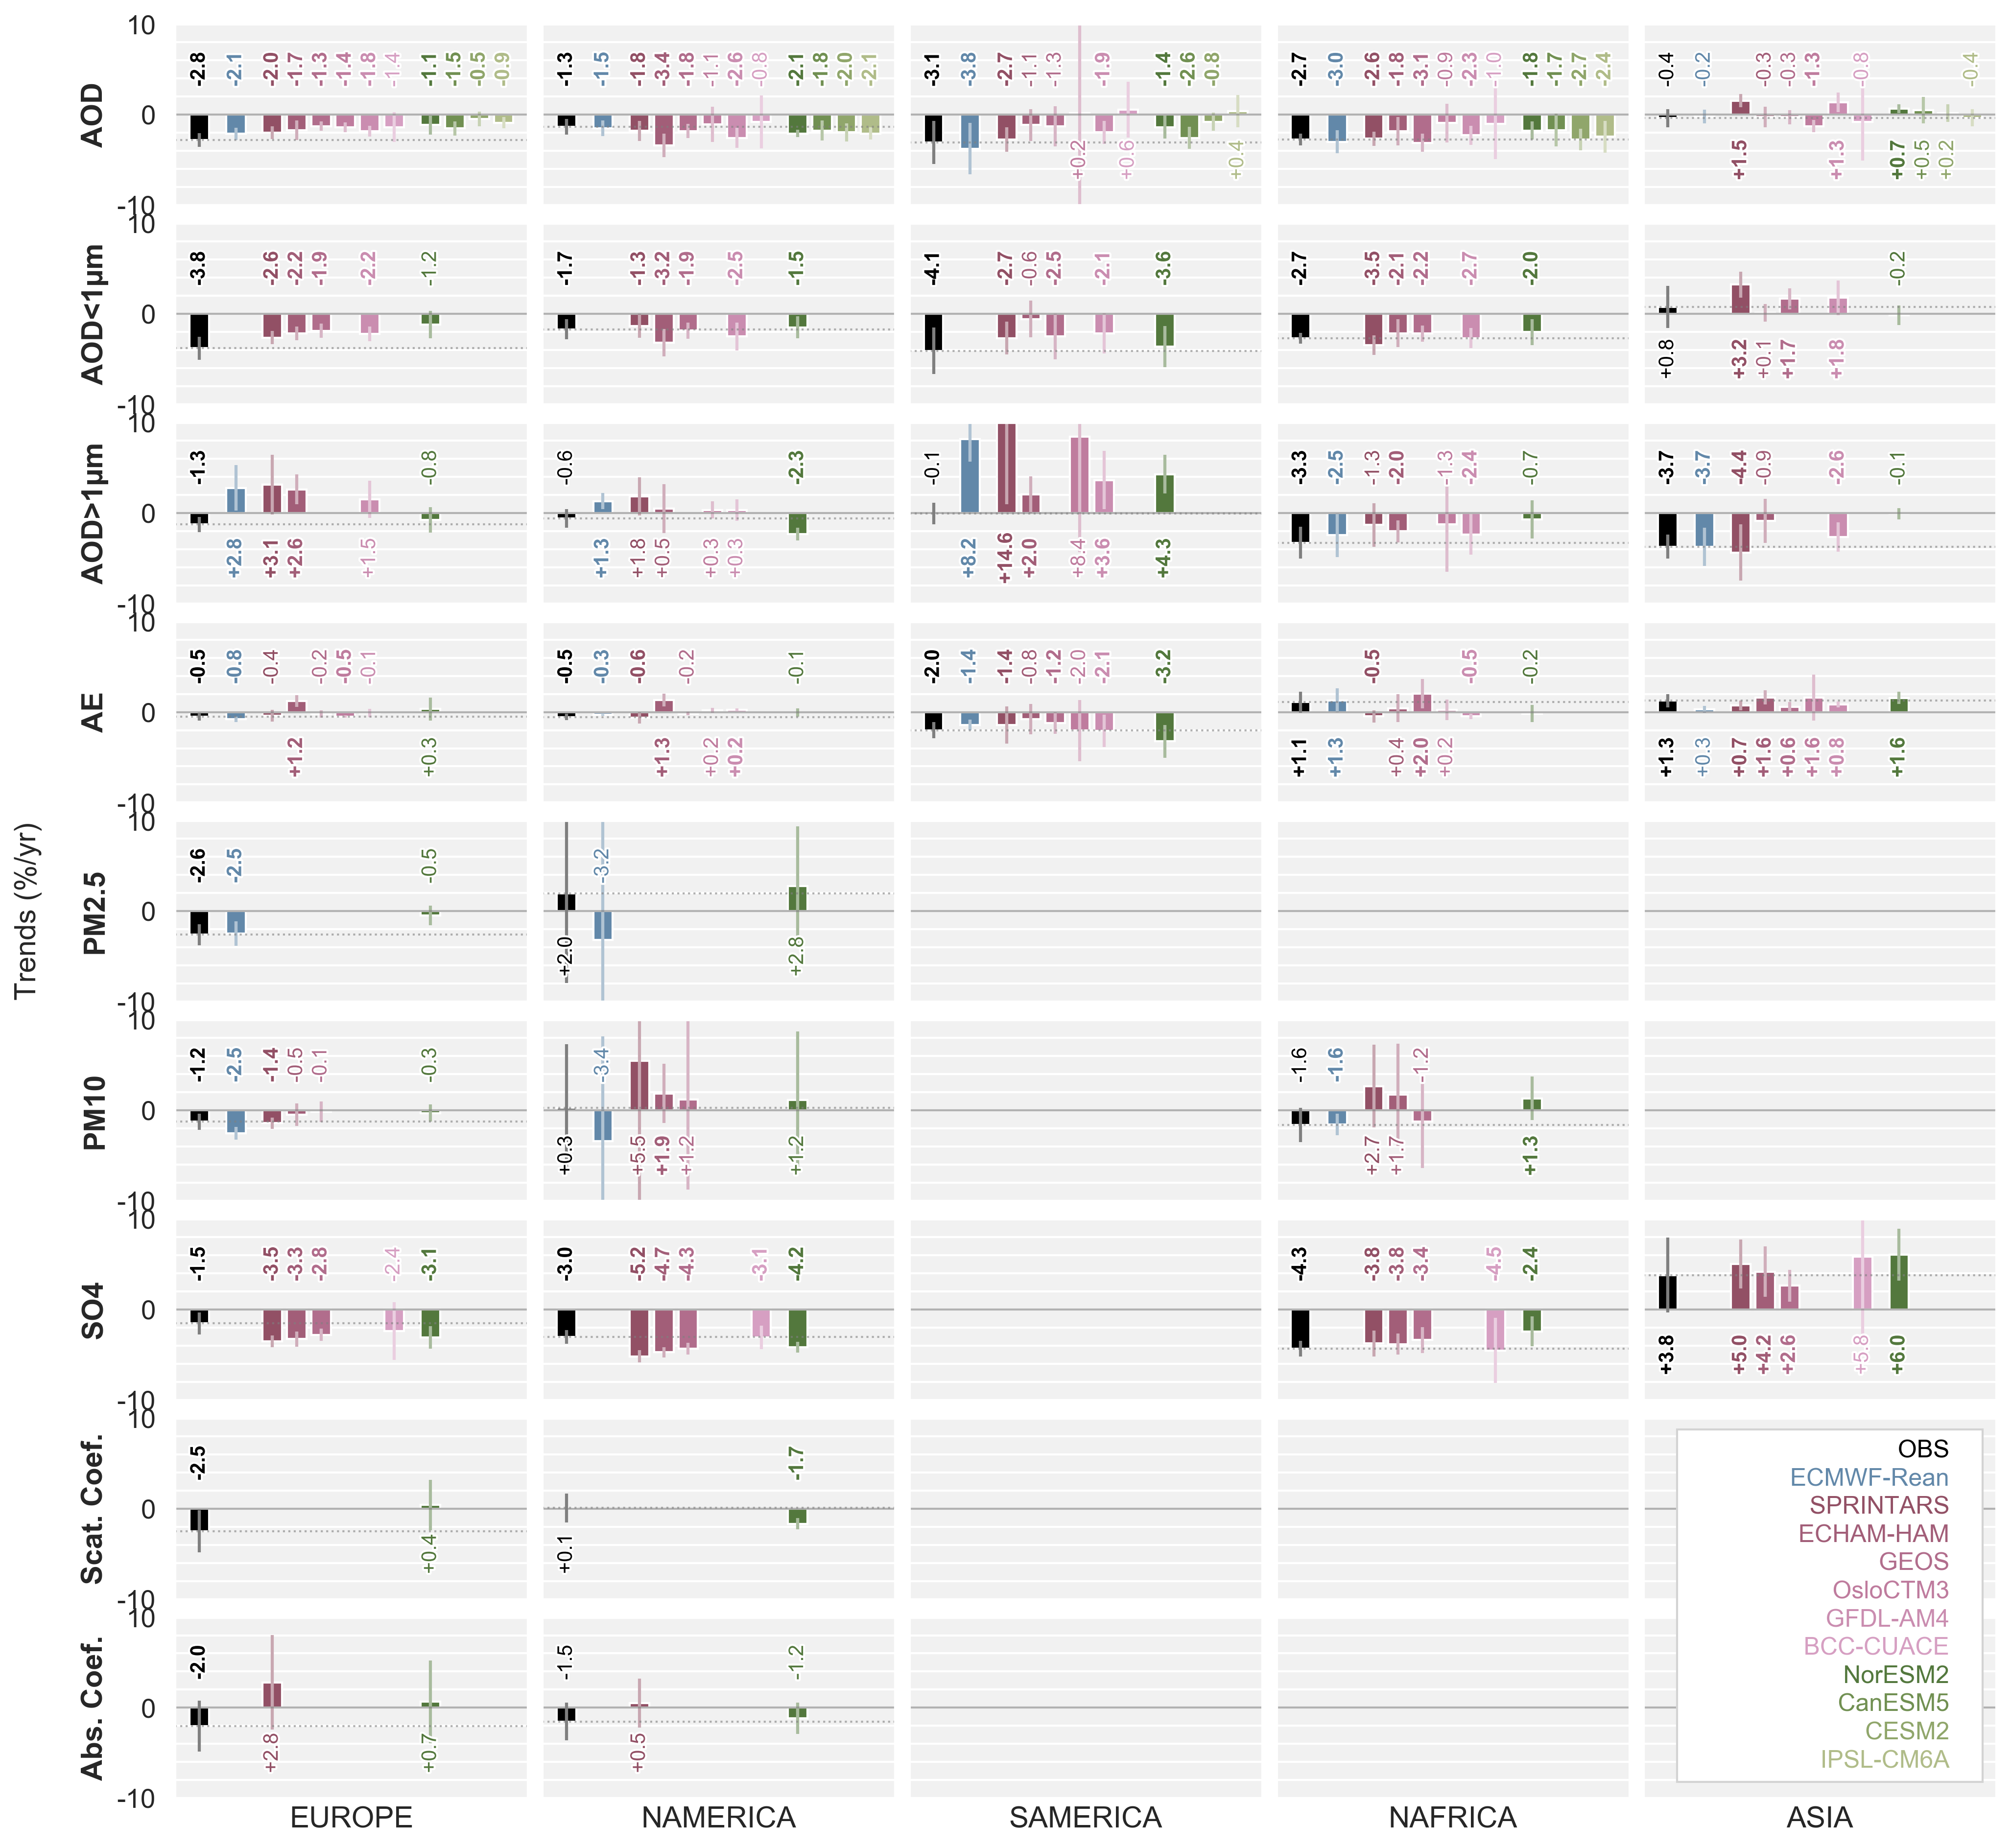
\includegraphics[width=16cm]{../scripts/figs/heatmaps/BARS.png}
 \caption{Regional trends of the aerosol properties computed with observations and models collocated in space and time to the observations. The error bars correspond to the uncertainty of the trend as calculated using both the uncertainty on the Theil−Sen slope and the residuals. The bold font indicates that the trends are significant with an expectancy of 95\% (p-val<0.05).}
 \label{fig:bars}
\end{figure}

In order to evaluate the trends from the models, the regional time series have been computed with the model output collocated in space and time to the available observations at the station level. The model trends are computed similar manner to the trends for the observation datasets. However, for the few models providing output every 5 years (in addition to 2014), the minimum required number of points has been reduced from 7 to 4, so the trends can be computed using the years 2000, 2005, 2010 and 2014. The results, shown in Figure \ref{fig:bars}, reveal different performances of the various models, for the reproduction of the observed trends, depending on the parameters and the regions.


\begin{itemize}
 \item AOD: the models show trends in the same direction as the observations over all the regions except in Asia, where the associated uncertainties are, however, usually larger than the trend values. Some differences between the three groups of models can be noticed when investigating the different regions:
       \begin{itemize}
        \item EUROPE: all the groups underestimate the observed decrease. With an average decrease of -1.0\%/yr, the CMIP6 models exhibit the highest underestimation, while the best performance is obtained with CAMS-Rean (-2.1\%/yr). The AP3 models trends range from -1.3\%/yr to -2.0\%/yr.
        \item NAMERICA: in contrast to the results for EUROPE, on average, all of the models overestimate the observed decrease in NAMERICA even though two models of the AP3 group simulate lower trends than found for observations. The consistency in the trends is very high within the CMIP6 group over this region.
        \item SAMERICA: CAMS Rean slightly overestimates the observed decrease while all the models of the two other groups underestimate this decrease. A few of the models capture positive trends, but these are associated with large uncertainties.
        \item NAFRICA: all the models capture the observed decreasing tendency. With a trend of -3.0\%/yr, CAMS-Rean is the closest to the observed trend (-2.7\%/yr). AP3 and CMIP6 multi-model trend averages are -2.0\%/yr and -2.2\%/yr, respectively.
        \item ASIA: A large inter-model variability is found in this region where the uncertainty is also significant. The means of the trends of each group range from -0.2\%/yr to +0.2\%/yr.
       \end{itemize}
 \item AOD<1µm: usually, the same patterns are found as for AOD. The models that underestimated the AOD underestimate AOD<1µm and vice versa. For AOD<1µm and the following parameters, only NorESM2 provides data for the CMIP6 group.
       \begin{itemize}
        \item in EUROPE: the underestimation of the decrease captured by the models is larger than the underestimation of AOD.
        \item ASIA: an increase, associated with large uncertainties is found in both models of the AP3 group (+1.3\%/yr) and observations (+0.8\%/yr).
       \end{itemize}
 \item AOD>1µm: the performance of the models is not as good as for AOD<1µm. This is also observed when evaluating the models for a single year \citep{jonaseval}. The inter model variability is also higher since some models simulate AOD>1µm trends in opposite directions in some regions.
       \begin{itemize}
        \item EUROPE: while the observations exhibit a significant decrease, CAMS-Rean and all of the AP3 models exhibit increasing values for AOD>1µm. NorESM2 from CMIP6 simulate a decrease consistent with the observations.
        \item SAMERICA: All of the models simulate large increases, from +4.3\%/yr up to +14.6\%/yr  which are not visible in the observations (-0.1\%/yr).
        \item NAFRICA: the models reproduce the observed decrease of 3.3\%/yr to some extent (from -0.7\%/yr to -2.5\%/yr). The fact that some 
        models with fixed SST (e.g ECHAM-HAM) reproduce this decrease does not support the hypothesis of the SST changes. The decrease in dust could be caused by increased wet scavenging of dust after coating with anthropogenic sulfate aerosols. The production of high levels of readily soluble materials on the dust surface makes indeed of dust aerosols effective cloud condensation nuclei \citep{fan2004impact,bauer2005impact,bauer2007sulfate,neubauer2019global}.
        \item ASIA: CAMS-Rean captures the same trend as computed with the observations dataset. Like for AOD<1µm, no certain trend can be identified  in this region with the CMIP6 model.
       \end{itemize}
 \item AE: the trends are usually relatively smaller than for AOD in the respective regions, meaning that the amount of the particles is more subject to variations than the size (type) of these particles. This feature is visible with both observations and models.
       \begin{itemize}
        \item EUROPE and NAMERICA: one model of the AP3 group (ECHAM-HAM) simulates a significant positive trend while negative tendencies are found in the observation and with the other models.
        \item SAMERICA: all of the models simulate negative trends, most of them significant, in agreement with the observations. CAMS-Rean and the AP3 models tend to underestimate the decrease, while the CMIP6 model tends to overestimate it.
        \item NAFRICA: CAMS-Rean reproduces well the observed increase (+1.3\%/yr VS +1.1\%/yr). The significant trends of the AP3 models range from -0.5\%/yr to +2.0\%/yr. The increase of AE supports the theory of enhanced scavenging of dust by anthropogenic aerosols.
        \item ASIA: the AP3 models and the CMIP6 model exhibit significant positive trends, which is also the case for the observations. CAMS-Rean does not capture any significant trend in this region.
       \end{itemize}
 \item $PM_{2.5}$: Almost all the models simulate significant decreases over Europe and North America, in good agreement with the observations. The CMIP6 model performs however better in North America, while it underestimates the extent of the decrease in Europe. Further analysis reveals that, despite the fact that it reproduces well the trend in North America, CAMS-Rean presents a large positive bias in this region (+100\%).
 \item $PM_{10}$: In North Africa, only CAMS-Rean reproduces the observed significant decrease. Positive trends are found for all the models of the AP3 and CMIP6 groups. As for $PM_{2.5}$, NorESM has better performance in North America. CAMS-Rean produces a trend as twice high as the observed trends both over Europe and North America.
 \item $SO_{4}$: The AP3 and CMIP6 models perform pretty well for the $SO_{4}$ surface concentration. The magnitude of the model trends is however higher than the observed trends in all the regions except North Africa.
 \item $\sigma_{sp}$ and $\sigma_{ap}$:  as mentioned in the previous section, the observations trends have been computed for these two parameters using data until 2018. The two models providing output for these parameters are NorESM2 and SPRINTARS. NorESM2 provides data until 2014, so the trends correspond to the period [2000-2014], while SPRINTARS provides data until 2018 and thus covers the whole observation period [2000-2018].
       \begin{itemize}
        \item EUROPE: a significant decrease is found in the observations for both $\sigma_{sp}$ and $\sigma_{ap}$ but is not captured by the models where positive trends are found, although associated with large uncertainties.
        \item NAMERICA: A significant decrease is found with NorESM2 for $\sigma_{sp}$ which is not seen in the observations. For Abs. Coef, NorESM2 captures a similar trend as derived from the observations, while SPRINTARS does not.
       \end{itemize}
\end{itemize}

This model trends evaluation reveals some key-points. Firstly, CAMS-Rean, which assimilates AOD, performs the best for capturing the trends of this parameter. Second, a large inter-model variability is generally found over Asia, where the observed trends are also the most uncertain.
Considering the total column, the models usually perform rather well for AOD, AOD<1µm, and AE, but show lower skill for AOD>1µm. At ground level, the models perform well for both $SO_{4}$ concentration and PM. The trends in $\sigma_{sp}$ and $\sigma_{ap}$ computed from regional time series are associated with large uncertainties due to the limited number of stations. This is exacerbated by the fact that data was only available from two models for these parameters.

\textcolor{red}{Can we identify significant differences between the model groups and link that to Table \ref{table:models}??}

\subsection{Trends in models}\label{global_trends}

\subsubsection{Global trends}

\begin{table}
 \begin{tabular}{lll}
  \tophline
                                & $Mean_{2000}$ & Trend (\%/yr) \\
  \middlehline
  AOD                           & (0.16) 0.14   & (+0.1) +0.2   \\
  AOD<1µm                       & (0.09) 0.05   & (+0.4) +0.6   \\
  AOD>1µm                       & (0.06) 0.09   & (-0.2) +0.1   \\
  AE                            & (0.78) 0.43   & (+0.2) +0.3   \\
  $PM_{2.5}$ (\unit{µg.m^{-3}}) & (12.4) 9.1    & (+0.2) +0.2   \\
  $PM_{10}$ (\unit{µg.m^{-3}})  & (19.3) 18.7   & (+0.1) +0.1   \\
  $SO_{4}$ (\unit{µg.m^{-3}})   & (2.33) 0.64   & (-1.1) +0.4   \\
  $\sigma_{sp}$ (\unit{Mm^{-1}})  & (28.0) 21.2   & (+0.3) +0.2   \\
  $\sigma_{ap}$ (\unit{Mm^{-1}})   & (3.1) 0.9     & (+1.8) +1.5   \\
  \bottomhline
 \end{tabular}
 \caption{Global means and trends of aerosol parameters using NorESM2 data. The value in parenthesis is obtained by aggregating only grid-points where observation stations are located while using the complete model time series. The relative trends are calculated by averaging the absolute trends within the considered grid-points and normalizing it to the global mean for the year 2000.}
 \label{table:global_trends}
\end{table}

\begin{figure}[t]
 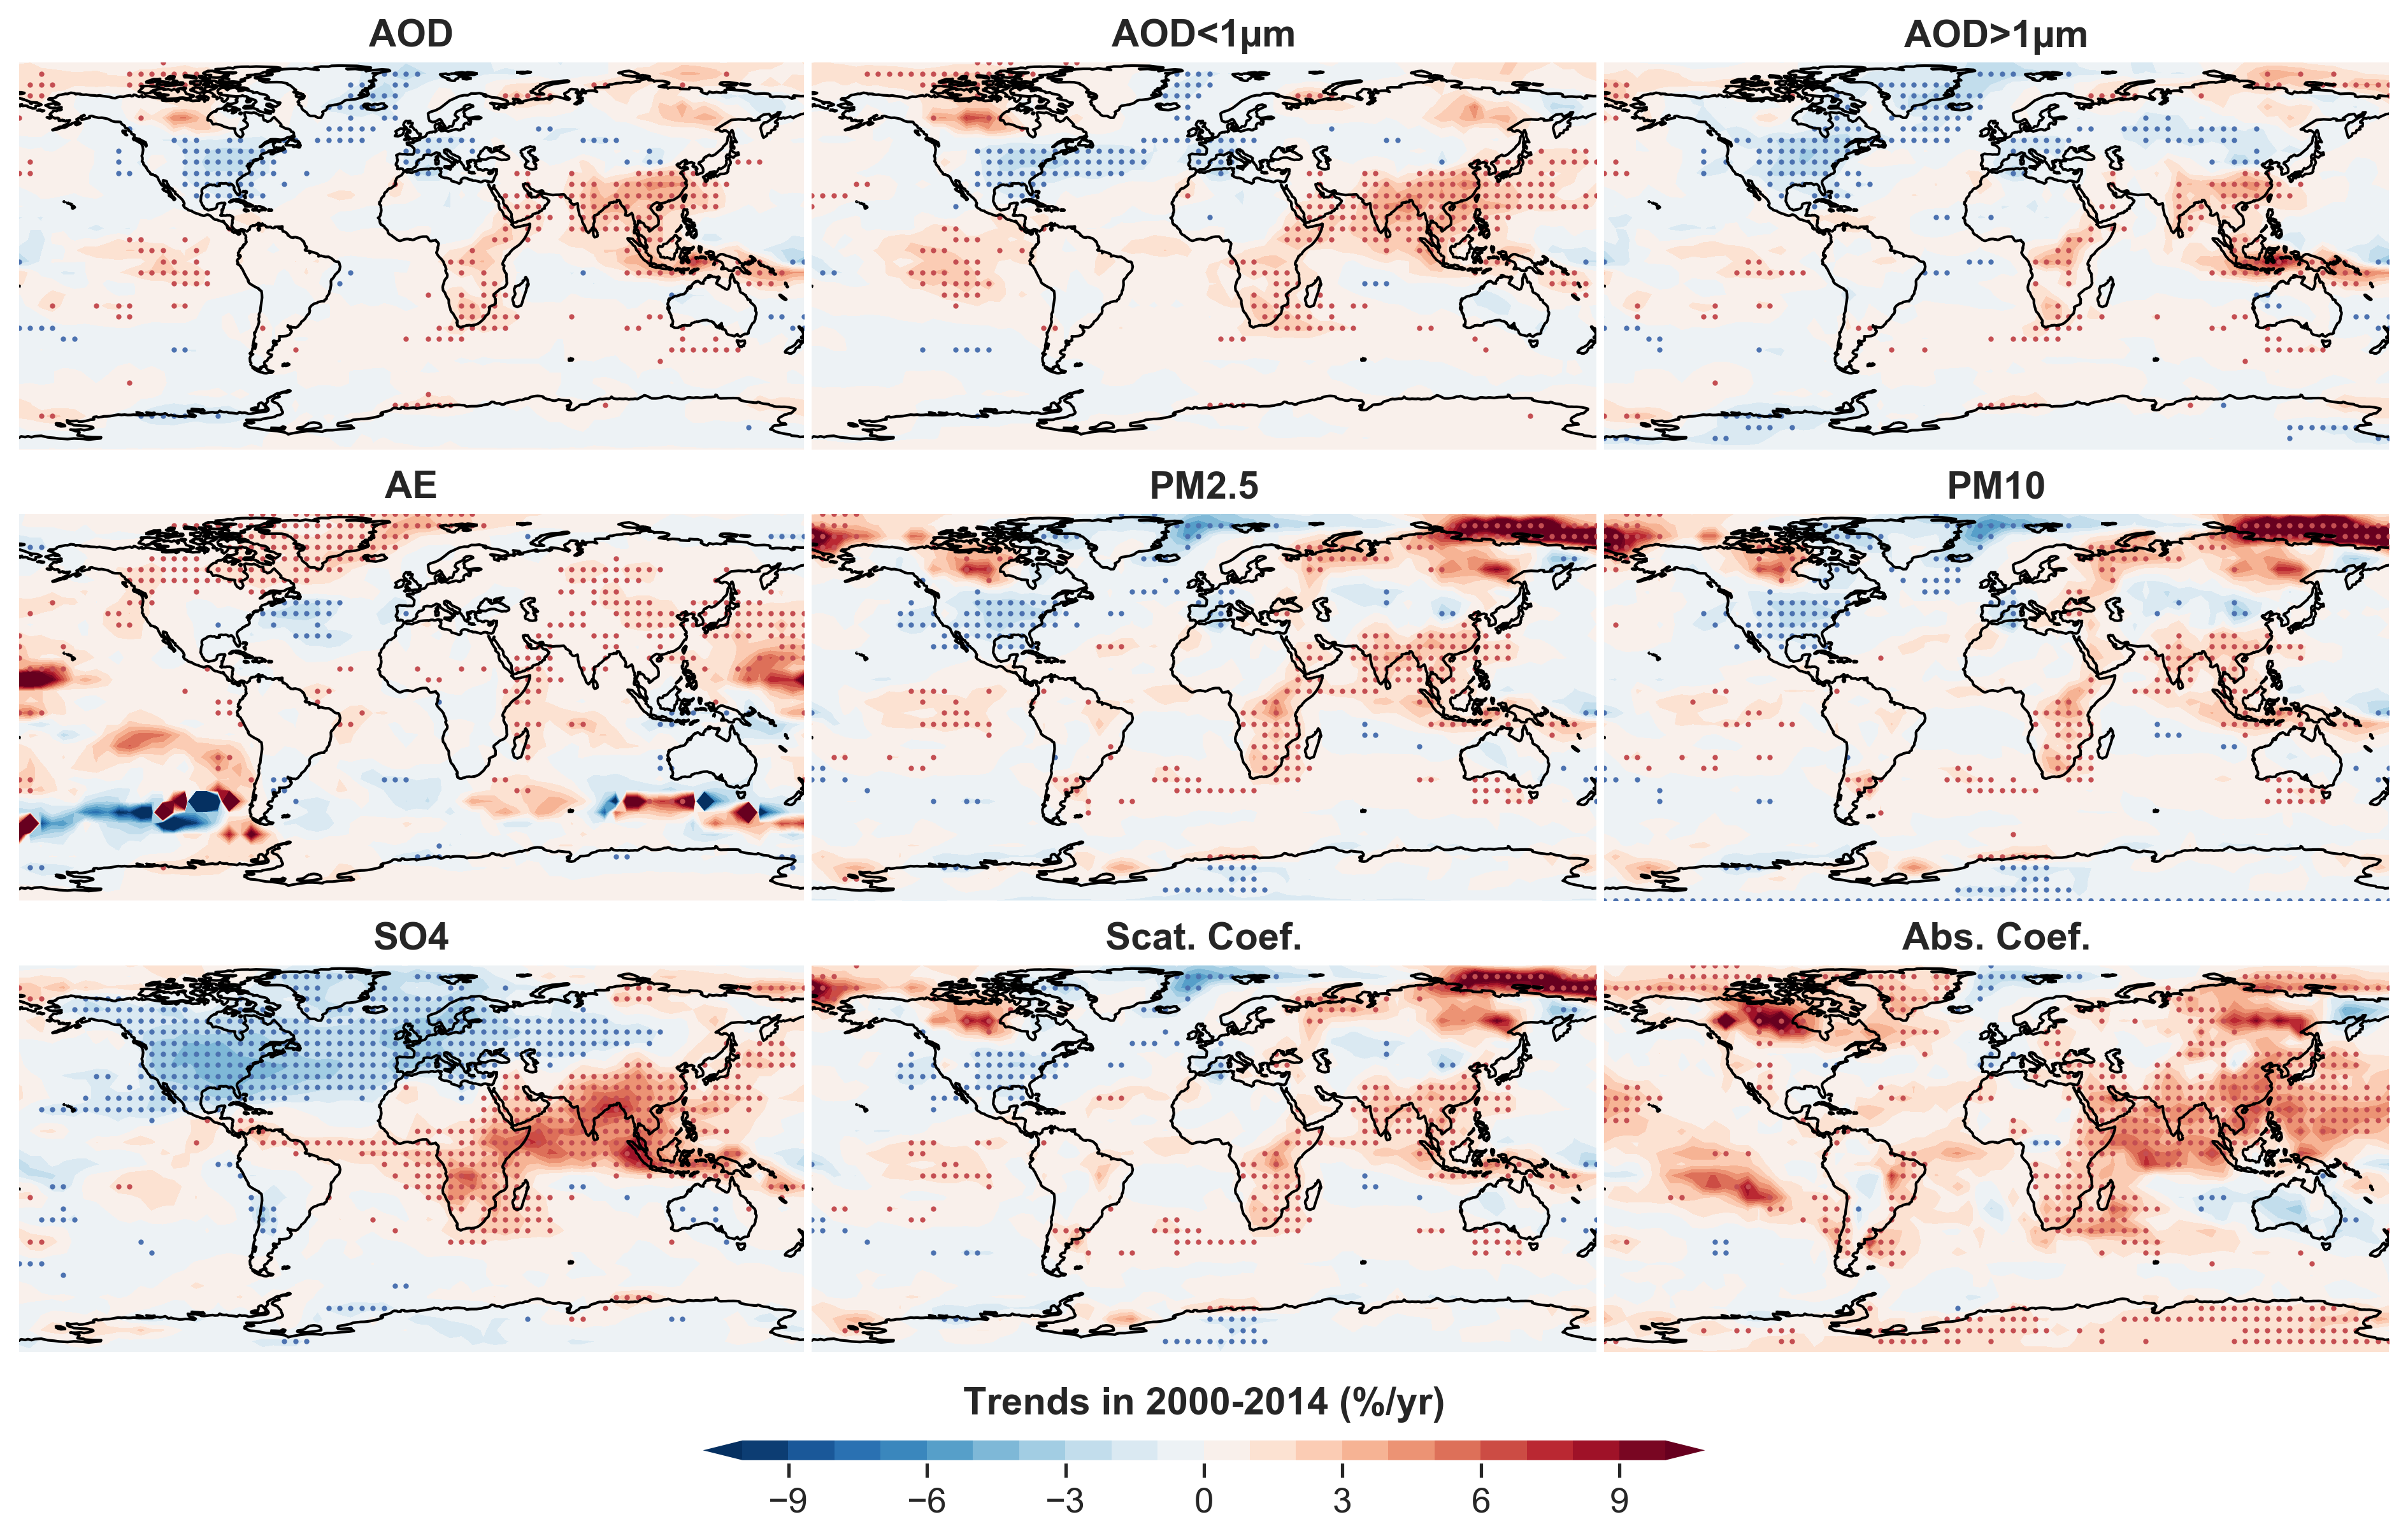
\includegraphics[width=16cm]{../scripts/figs/trends_map2.png}
 \caption{Global trends of aerosol properties using NorESM2 data regridded at a 5x5 degrees resolution. The blue and red dots dots indicate respectively significant negative and positive trends.}
 \label{fig:global_trends}
\end{figure}

As discussed previously, the regional trends are not always representative of the trends happening in the extended regions and over the whole study period. The reasons are the partial spatial and time coverage of the ground based observations. Moreover, the observation stations are obviously located over land. This does not allow for depiction of a global picture of the aerosol trends, and is unfortunate as sea salt particles are among the most predominant aerosols on Earth \citep{schulz2004sea}.

In order to provide an assessment of the aerosol trends at a global scale, we present, in this section, the trends computed with the NorESM2 data (CMIP6 group) using all grid boxes. The calculation of the global trend is made by averaging the absolute trends computed at each grid-point of the model. In order to provide a relative trend, this absolute trend is normalized to the global average of the considered parameter for the year 2000. The global trends are reported for the nine aerosol parameters in Table \ref{table:global_trends}. The global maps, shown in Figure \ref{fig:global_trends}, enable investigation of the spatial variability of these trends.

While the observed trends of the three AOD parameters show a decrease in most of the regions of the World, the global AOD trend is actually positive (+0.2\%/yr). This global increase is also found with other models. Averages of the models from the CAMS-Rean and the AP3 groups simulate global trends of about +0.2\%/yr and +0.3\%/yr respectively. Within the CMIP6 group, IPSL and CESM2 also exhibit positive trends (+0.7\%/yr and +0.3\%/yr), consistent with NorESM2, while CanESM simulates a negative trend (-0.8\%/yr). The relative increase of 0.2\%/yr found with NorESM2 corresponds to an absolute rate of +0.0028/decade, which is in perfect agreement with the global trend (over the oceans) of +0.003/decade reported by \cite{zhang2010decadal} using MODIS data. The increase of AOD is observed to be larger for the fine fraction, with an increase of about +0.6\%/yr, as compared to +0.1\%/yr for AOD>1µm. As seen in Figure \ref{fig:global_trends}, similar geographical patterns are found for the three AODs: increase in South-Africa and East-Asia and decrease in Europe and in the US. The increasing AOD observed in Canada is dominated by an increase of AOD<1µm in this region. The important increase of AOD in Indonesia seems to be linked to a large increase of AOD>1µm. Over the Pacific Ocean, one region has significant positive modelled trends in both AOD and AOD<1µm. Almost no significant trend is found south of 60\textdegree S.

The model also simulates an increase for AE on a global scale, with a rate of +0.3\%/yr. This suggests a shift towards smaller particles. The largest increases are found over Canada, Greenland, Siberia and the Pacific Ocean. There are some distinct outliers around 60\textdegree S. In the Atlantic, we find a decrease of AE, which is consistent with the decrease of AOD<1µm in the same region.

The trends in both $PM_{2.5}$ and $PM_{10}$ exhibit similar geographical features as for AOD. In addition, one finds large and significantly increasing trends in the high Arctic. The global averages show that $PM_{2.5}$ is increasing faster than $PM_{10}$  (+0.2\%/yr vs. +0.1\%/yr), which is consistent with the increasing AE, suggesting a relatively higher fraction of fine particles with time.

The surface $SO_{4}$ concentration trends map reveals two large contrasting regions. Significant decreases are found over North America and Europe, while significant increases are found over southern and eastern Asia and southern to central parts of Africa. This illustrates the shift of polluting activities from the developed countries to the developing countries during the last two decades. With an overall increase of +0.4\%/yr, the global trend is positive.

The $\sigma_{sp}$ trends are very similar to those observed for both $PM_{2.5}$ and $PM_{10}$. The same geographical patterns are found, as well as the global average trend which amounts to an increase of 0.2 \%/yr over the study period.

$\sigma_{ap}$ reveals increasing tendencies over most of the grid-boxes of the model, except in Europe, Eastern part of US an Australia, which explains why the largest global trend is obtained for this parameter, with an average of +1.5\%/yr. Further analysis shows that this increase is related to an increase of the BC fraction of the AOD rather homogeneously in space with, nevertheless, a hot spot in East-Asia. A global trend of +2.3\%/yr is found for the BC OD (Optical Depth).

Table \ref{table:global_trends} also contains the trends computed for the different aerosol parameters when combining only the grid-points where an observation station is located, whether measurements are available or not. Significant differences in 'global' trends can be found when observations are not provided over some regions. This is most obvious for $SO_{4}$ for which the observation stations are located mostly in Europe and North America and exhibit decreasing values, while only a few stations are located in the regions associated with increasing values. In this case, the computation of the trends by considering only observation station grid-boxes leads to a global decrease of -1.1\%/yr while consideration of all of the grid-boxes of the model leads to a global increase of +0.4\%/yr.


\subsubsection{Contribution of main aerosol species to the AOD trends}

\begin{figure}[t]
 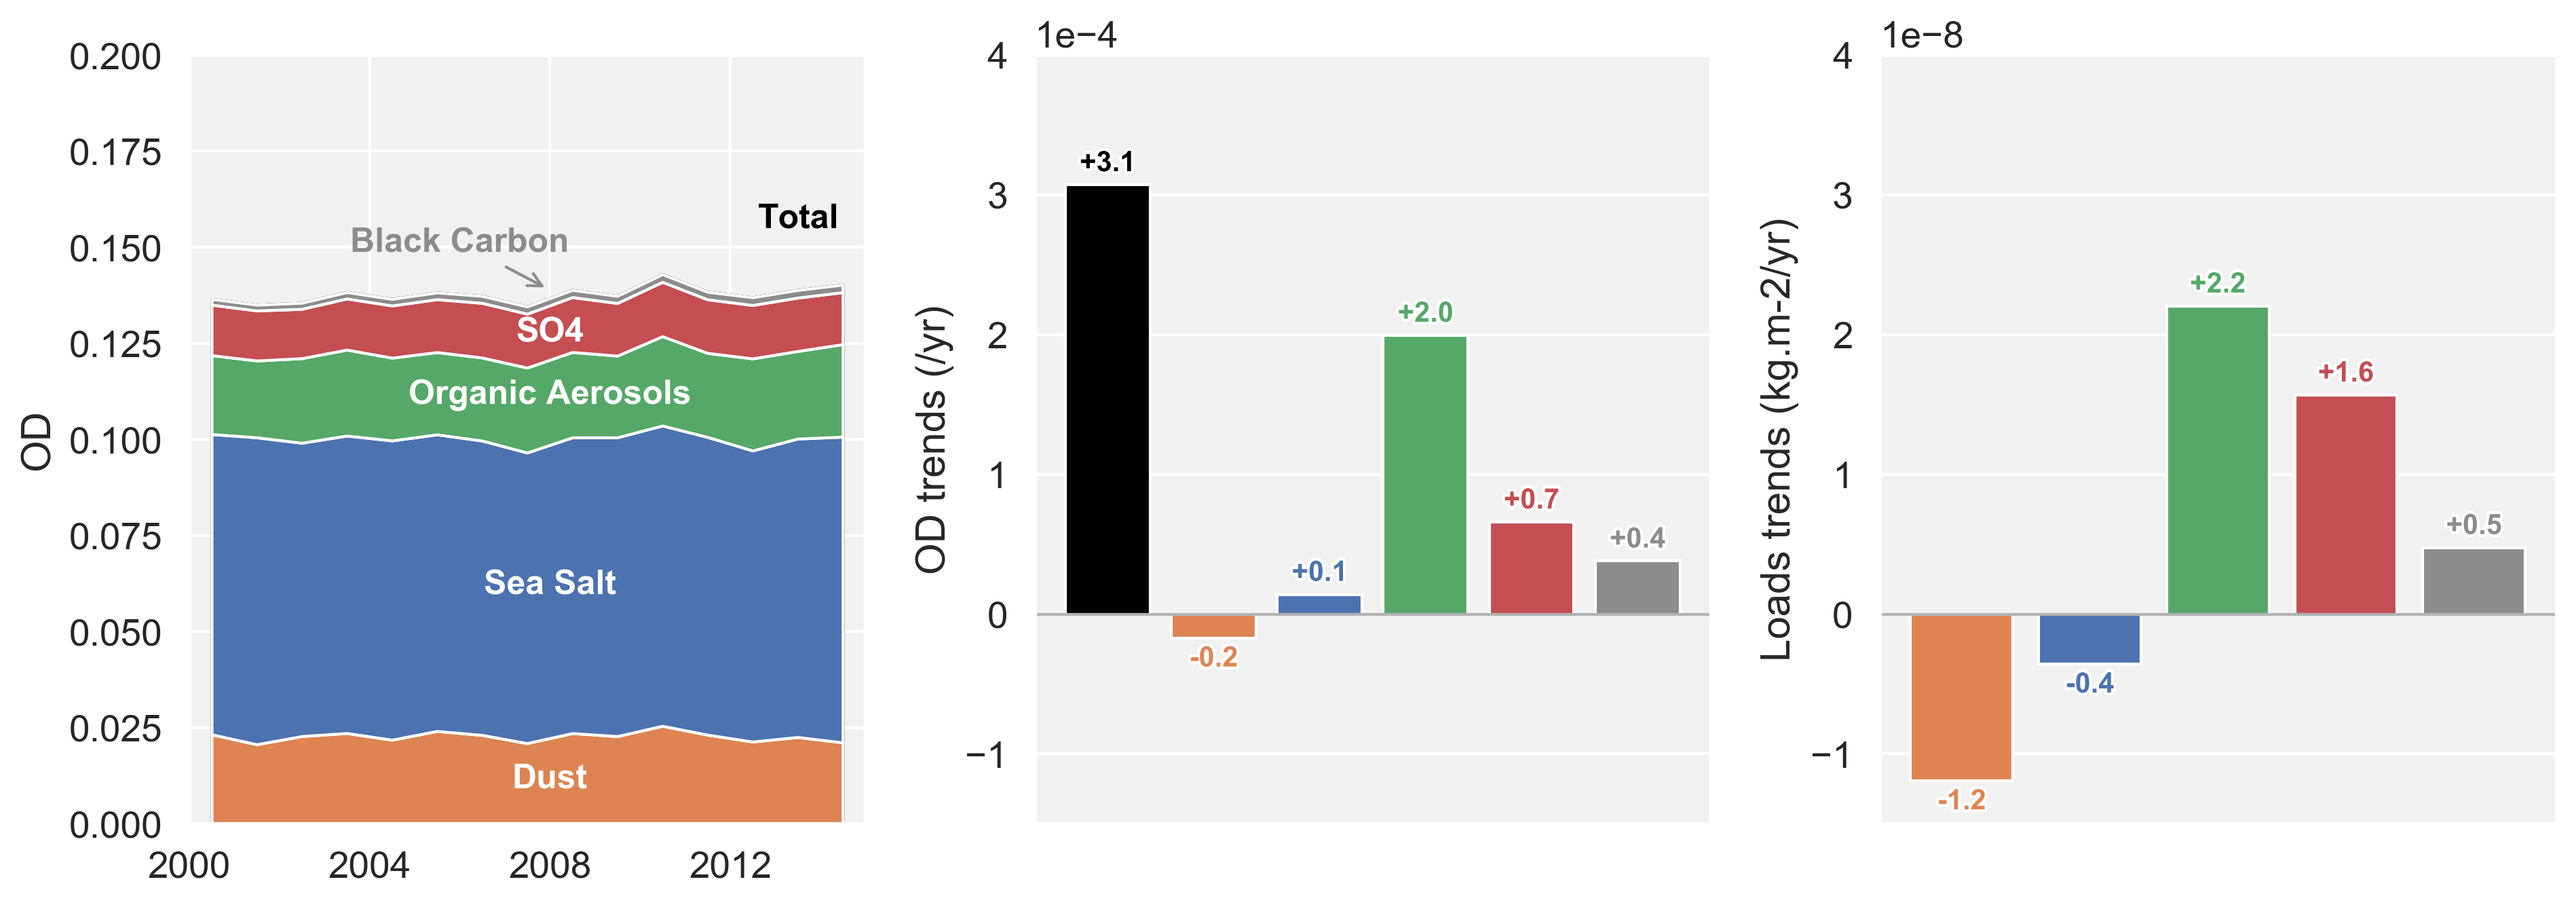
\includegraphics[width=16cm]{../scripts/figs/abs_species_trends.png}
 %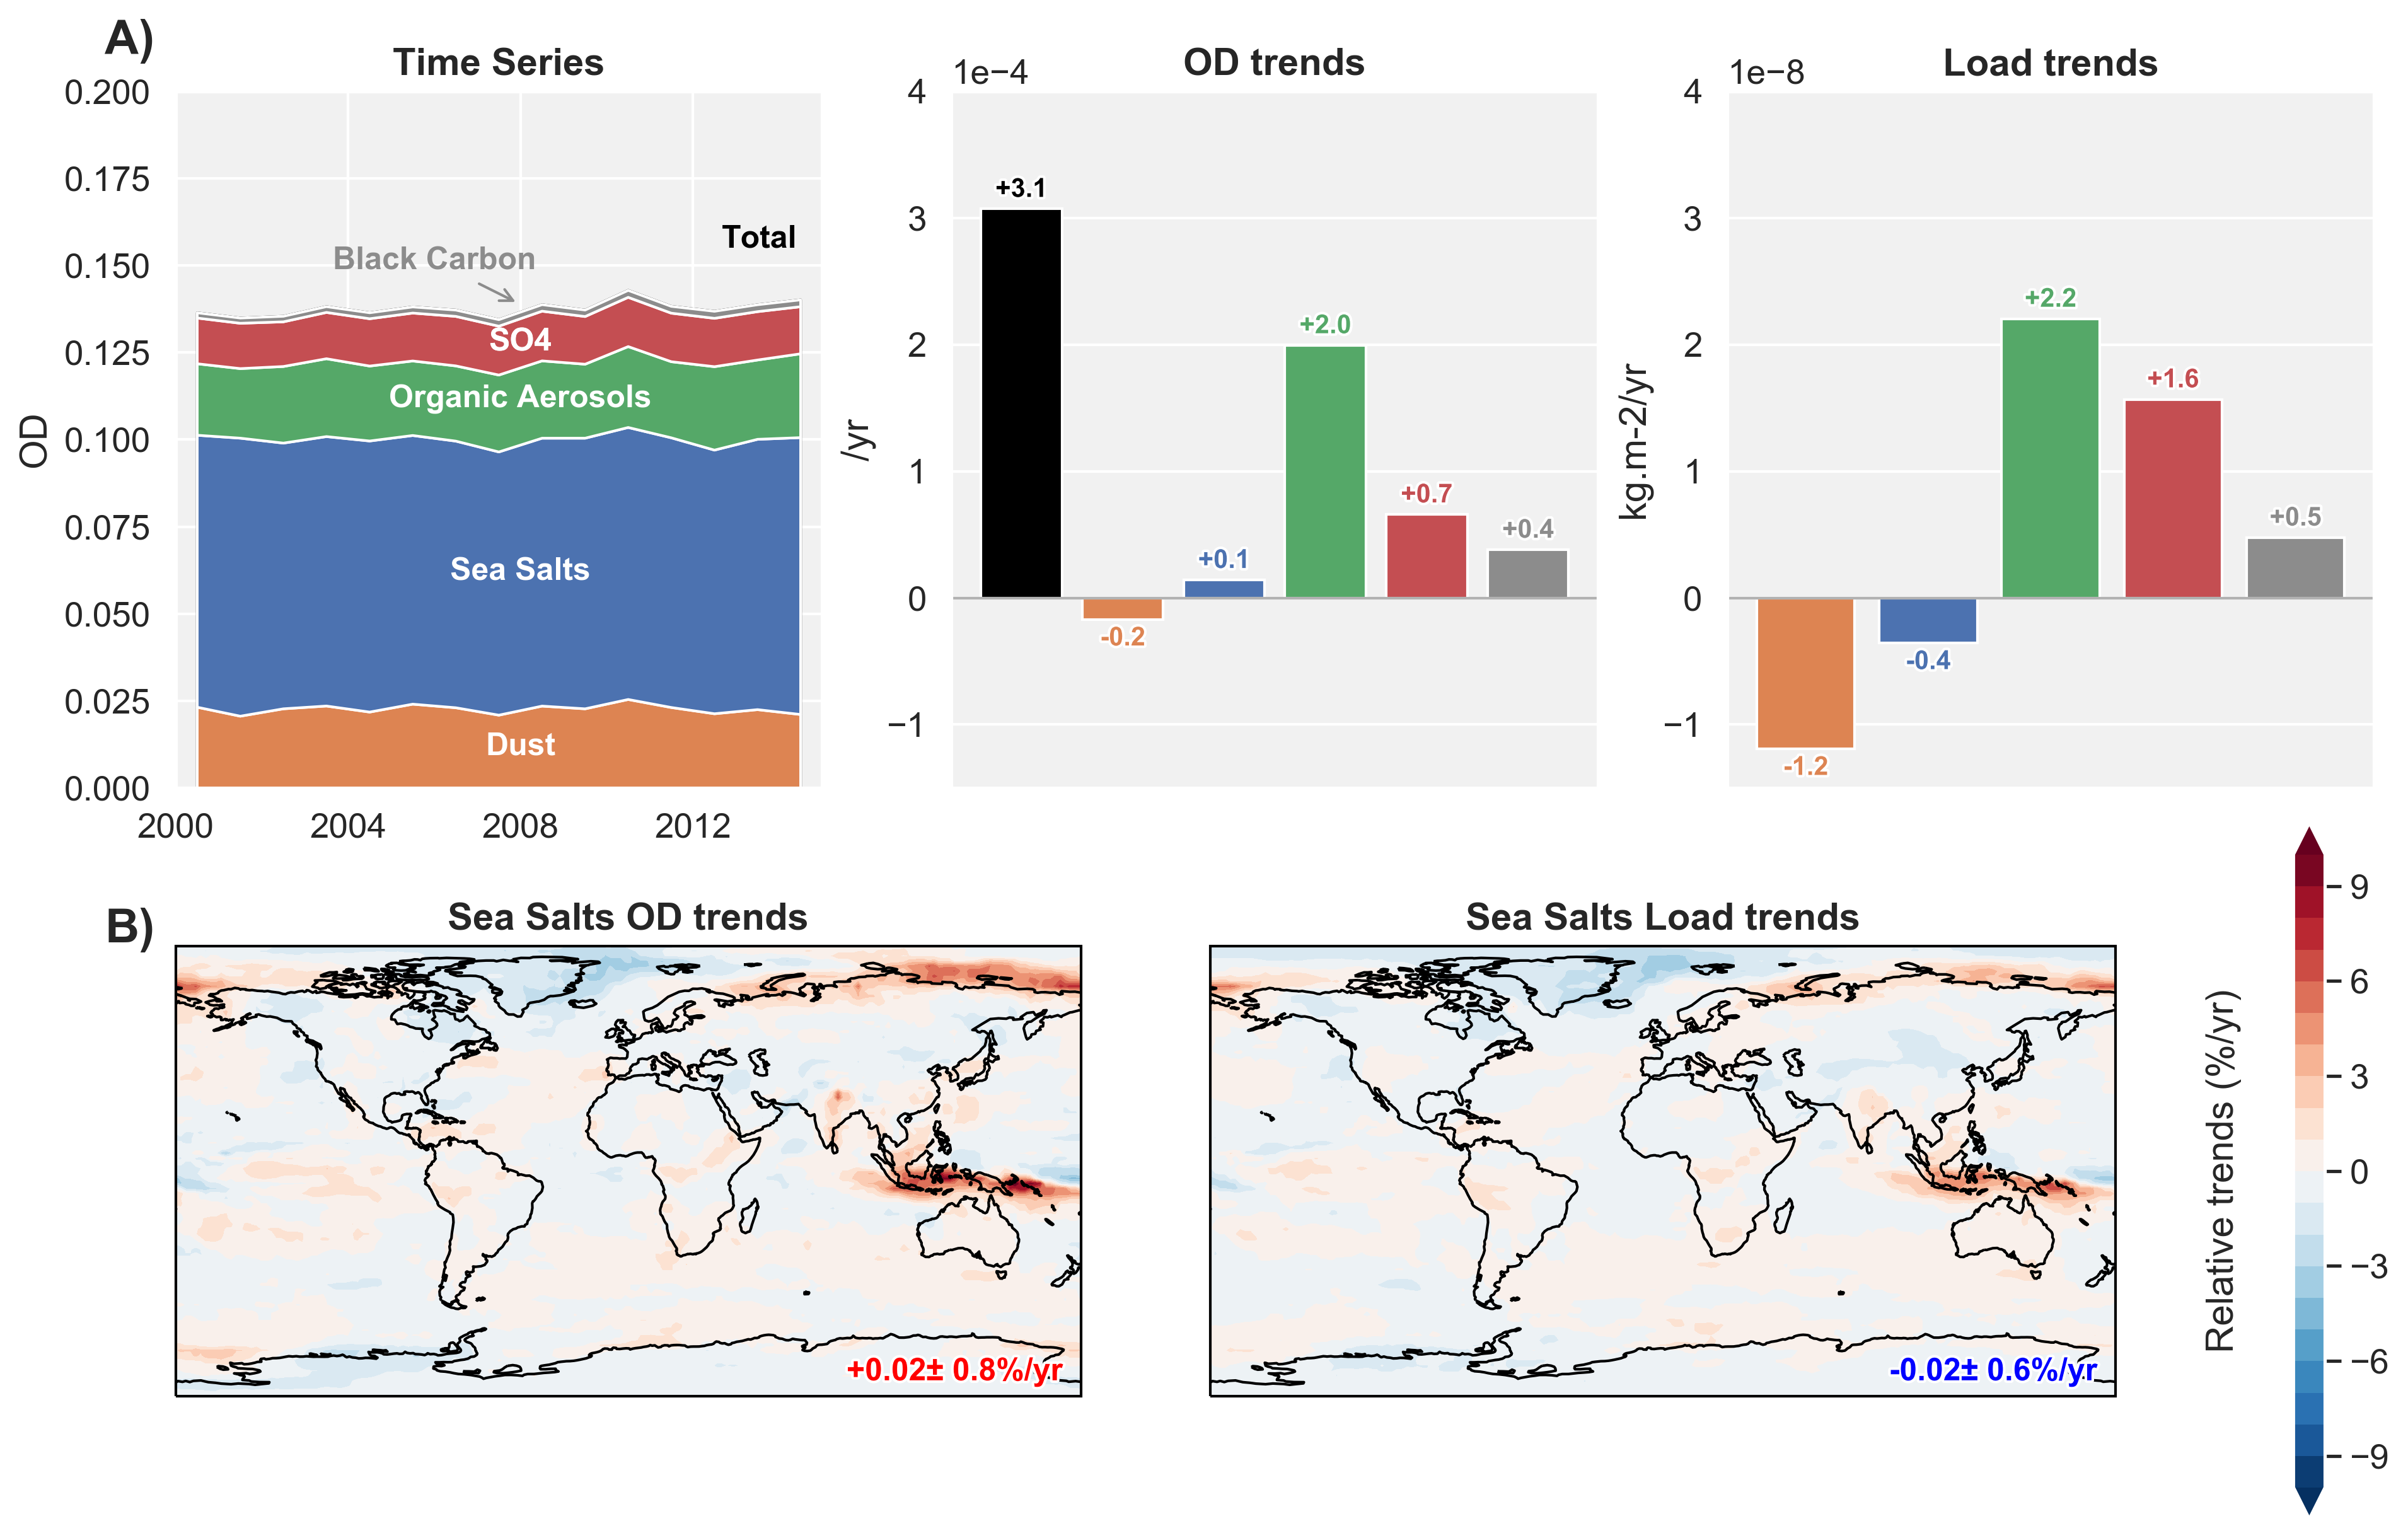
\includegraphics[width=16cm]{../scripts/figs/pannel-abs_species_trends.png}
 \caption{Absolute trends in OD and emissions of the main aerosol species computed with NorESM2. The y-axis of the trends in OD and the emissions is given according to the power of 10 indicated at the top left corner of each of the subplots.}
 \label{fig:species}
\end{figure}

The averaged global trend computed by NorESM2 indicates an increase of AOD in the 2000-2014 period with a rate of about 0.2\%/yr. The trends in AE, AOD<1µm and AOD>1µm indicate that the fine particles are primarily responsible for this increase in the atmospheric column.

In this section, we investigate the trends of the major aerosol species simulated by NorESM2. For that purpose, the absolute trends of the individual contribution of these species to the AOD were computed, as well as the trends in the loads and the emissions. The trends of OD and loads are shown in Figure \ref{fig:species}. In this version, NorESM2 simulates a large proportion of sea salt. This is the result of a model tuning used for reaching climate equilibrium. While the model attributes too much OD to SS, the trends should not be affected by this tuning.

The relative increase of AOD of +0.2\%/yr corresponds to an absolute increase of +3.1 e \unit{^{-4}/yr}. This positive trend is dominated by an increase of the Organic Aerosols (OA), $SO_{4}$ and Black Carbon, which are responsible for an increase of the OD of about +2.0 e \unit{^{-4}/yr}, +0.7 e \unit{^{-4}/yr} and +0.4e \unit{^{-4}/yr}, respectively. The relative OD trends give a different ranking since the highest increase is found for BC (+2.5\%/yr), followed by OA (+0.5 \%/yr). On average, the contribution of dust and sea salt is slightly negative (-0.1 \unit{^{-4}/yr}).

The trends in OD do not necessarily represent the trends in the aerosol loads, since the different species have different mass extinction coefficients (from this study, dust: 1.8 \unit{m^{2}.g^{-1}}, SS: 4.3 \unit{m^{2}.g^{-1}}, OA: 5.6 \unit{m^{2}.g^{-1}}, $SO_{4}$: 5.3 \unit{m^{2}.g^{-1}}, BC: 7.6 \unit{m^{2}.g^{-1}}). For sea salt, opposite trends are even observed for the sea salt OD (positive trend) and the sea salt load (negative trend). The analysis of the global maps (not shown in this study) reveals that the largest increases of the sea salt load  happen in Indonesia and near the North Pole and result in a relatively larger increase of OD in these areas. This effect relates to the higher relative humidity at these latitudes which makes the sea salt, which is very hygroscopic, more efficient at light extinction.


\conclusions  %% \conclusions[modified heading if necessary]

The main findings of this multi parameter trends analysis can be listed as follows:
\begin{itemize}
 \item The observations depict mostly negative trends regarding the extensive parameters in the different regions of the World. In Asia, AE is increasing in time consistent with AOD<1µm and $SO_{4}$, which reflects the regional increase of the anthropogenic aerosols in that region.
 \item Some observation networks allow for the derivation of representative trends over the whole study period. In other cases, the partial time and space coverage of the observations can induce artificial trends when using regional time series.
 \item The models tend to capture observed AOD, AE, $SO_{4}$ and PM trends but show larger discrepancies regarding AOD>1μm. The lower amount of data for Scat. and $\sigma_{ap}$ makes the validation of the modeled trends more uncertain.
 \item The global trends computed using model data give a different picture than the trends obtained when using only ground-based observations.
 \item The global trends computed with the model data show mostly positive trends for all the extensive parameters. The trends in AOD are dominated by the increase of the fine particles both in the column and at the surface. This tendency to finer particles is also found with the positive trend in AE. This increase appears to be dominated by the organic aerosols, for which the emissions have increased in the study period, and by the $SO_{4}$ whose emissions were shifted from Europe and North America to Africa and East-Asia where a global positive $SO_{4}$ trend is found.
\end{itemize}

Some elements were not considered in this study which could be investigated in order to complete the aerosol trends picture:
\begin{itemize}
 \item Some regions are associated with strong seasonal cycles. In South America, the regional time series shows high peaks in AOD, associated with forest fires in the late summer, whose intensity greatly varies from year to year. In Africa, a strong seasonal contrast is also found due to the transport of desert dust at altitude in the summer months \citep{mortier2016, ogunjobi2008synoptic}. The computation of the seasonal trends would allow characterization of the tendencies in such extreme or synoptic aerosol events.
 \item  This study shows that the trends computed from the ground-based observations networks are not representative of the global aerosol trends due to the inhomogeneities in data spatial coverage. The satellites providing a global Earth observation could be utilized for the evaluation of the model trends in the regions lacking observations and over the oceans \citep{hsu2012global,zhang2010decadal}.
 \item The trends in the meteorological parameters could be investigated in parallel with the aerosol trends because they affect the aerosols life cycle and their optical properties \citep{che2019large}. Hypothetical trends in wind velocity could produce trends in the loads of sea salt and dust and, as seen in the last section, trends in OD could be enhanced by relative humidity changes. Also, changes in temperature could impact the magnitude of the biogenic emissions. Increasing temperatures, associated with changes in land use and high atmospheric CO2 concentrations have been shown to lead to an increase of the BVOC emissions \citep{penuelas2010bvocs}. Finally, trends in precipitation that are responsible for aerosol wet scavenging would directly produce trends in aerosol loads.
 \item Several studies have linked the trends in anthropogenic aerosols to radiative forcing variations while investigating sources of global dimming and brightening \cite{streets2006two,norris2007trends}. It could be of interest to evaluate how much the modeled trends deviations, as compared to the observations, are affecting the calculation of the radiative forcing, in the different regions of the World, and at a global scale.
 \item While assembling the dataset for this analysis, it appeared that more models and observations ($\sigma_{ap}$ in the US) could be utilized. Due to time limitations, these data could not be integrated in the study, but could be considered in the future to enrich both databases.
 \item \textcolor{red}{could use model pressure levels to include mountain sites which are often impacted by transport??}
\end{itemize}


%% The following commands are for the statements about the availability of data sets and/or software code corresponding to the manuscript.
%% It is strongly recommended to make use of these sections in case data sets and/or software code have been part of your research the article is based on.

\codeavailability{TEXT} %% use this section when having only software code available

The observation and model data were read and collocated with the pyaerocom python library (\url{https://github.com/metno/pyaerocom}, version 0.8.0).

%\dataavailability{TEXT} %% use this section when having only data sets available


%\codedataavailability{TEXT} %% use this section when having data sets and software code available


%\sampleavailability{TEXT} %% use this section when having geoscientific samples available


%\videosupplement{TEXT} %% use this section when having video supplements available


%\appendix
%\section{} %\label{sec:representativity} %% Appendix A

%\subsection{}     %% Appendix A1, A2, etc.


%\noappendix       %% use this to mark the end of the appendix section

%% Regarding figures and tables in appendices, the following two options are possible depending on your general handling of figures and tables in the manuscript environment:

%% Option 1: If you sorted all figures and tables into the sections of the text, please also sort the appendix figures and appendix tables into the respective appendix sections.
%% They will be correctly named automatically.

%% Option 2: If you put all figures after the reference list, please insert appendix tables and figures after the normal tables and figures.
%% To rename them correctly to A1, A2, etc., please add the following commands in front of them:


%\appendixfigures  %% needs to be added in front of appendix figures

%\appendixtables   %% needs to be added in front of appendix tables

%% Please add \clearpage between each table and/or figure. Further guidelines on figures and tables can be found below.

\authorcontribution{TEXT} %% this section is mandatory

\competinginterests{TEXT} %% this section is mandatory even if you declare that no competing interests are present
No competing interests.

%\disclaimer{TEXT} %% optional section

\begin{acknowledgements}
 Data providers from all the regional and global networks are greatly acknowledged for sharing and submitting their data to be used. DN acknowledges funding from the European Union’s Horizon 2020 research and innovation programme project FORCeS under grant agreement No 821205.
\end{acknowledgements}




%% REFERENCES

%% The reference list is compiled as follows:

%\begin{thebibliography}{}

% \bibitem[AUTHOR(YEAR)]{LABEL1}
% REFERENCE 1

% \bibitem[AUTHOR(YEAR)]{LABEL2}
% REFERENCE 2

%\end{thebibliography}

%% Since the Copernicus LaTeX package includes the BibTeX style file copernicus.bst,
%% authors experienced with BibTeX only have to include the following two lines:
%%
\bibliographystyle{copernicus}
\bibliography{mybib.bib}
%%
%% URLs and DOIs can be entered in your BibTeX file as:
%%
%% URL = {http://www.xyz.org/~jones/idx_g.htm}
%% DOI = {10.5194/xyz}


%% LITERATURE CITATIONS
%%
%% command                        & example result
%% \citet{jones90}|               & Jones et al. (1990)
%% \citep{jones90}|               & (Jones et al., 1990)
%% \citep{jones90,jones93}|       & (Jones et al., 1990, 1993)
%% \citep[p.~32]{jones90}|        & (Jones et al., 1990, p.~32)
%% \citep[e.g.,][]{jones90}|      & (e.g., Jones et al., 1990)
%% \citep[e.g.,][p.~32]{jones90}| & (e.g., Jones et al., 1990, p.~32)
%% \citeauthor{jones90}|          & Jones et al.
%% \citeyear{jones90}|            & 1990



%% FIGURES

%% When figures and tables are placed at the end of the MS (article in one-column style), please add \clearpage
%% between bibliography and first table and/or figure as well as between each table and/or figure.


%% ONE-COLUMN FIGURES

%%f
%\begin{figure}[t]
%\includegraphics[width=12cm]{FILE NAME}
%\caption{TEXT}
%\end{figure}
%
%%% TWO-COLUMN FIGURES
%
%%f
%\begin{figure*}[t]
%\includegraphics[width=16cm]{FILE NAME}
%\caption{TEXT}
%\end{figure*}
%
%
%%% TABLES
%%%
%%% The different columns must be seperated with a & command and should
%%% end with \\ to identify the column brake.
%
%%% ONE-COLUMN TABLE
%
%%t
%\begin{table}[t]
%\caption{TEXT}
%\begin{tabular}{column = lcr}
%\tophline
%
%\middlehline
%
%\bottomhline
%\end{tabular}
%\belowtable{} % Table Footnotes
%\end{table}
%
%%% TWO-COLUMN TABLE
%
%%t
%\begin{table*}[t]
%\caption{TEXT}
%\begin{tabular}{column = lcr}
%\tophline
%
%\middlehline
%
%\bottomhline
%\end{tabular}
%\belowtable{} % Table Footnotes
%\end{table*}
%
%%% LANDSCAPE TABLE
%
%%t
%\begin{sidewaystable*}[t]
%\caption{TEXT}
%\begin{tabular}{column = lcr}
%\tophline
%
%\middlehline
%
%\bottomhline
%\end{tabular}
%\belowtable{} % Table Footnotes
%\end{sidewaystable*}
%
%
%%% MATHEMATICAL EXPRESSIONS
%
%%% All papers typeset by Copernicus Publications follow the math typesetting regulations
%%% given by the IUPAC Green Book (IUPAC: Quantities, Units and Symbols in Physical Chemistry,
%%% 2nd Edn., Blackwell Science, available at: http://old.iupac.org/publications/books/gbook/green_book_2ed.pdf, 1993).
%%%
%%% Physical quantities/variables are typeset in italic font (t for time, T for Temperature)
%%% Indices which are not defined are typeset in italic font (x, y, z, a, b, c)
%%% Items/objects which are defined are typeset in roman font (Car A, Car B)
%%% Descriptions/specifications which are defined by itself are typeset in roman font (abs, rel, ref, tot, net, ice)
%%% Abbreviations from 2 letters are typeset in roman font (RH, LAI)
%%% Vectors are identified in bold italic font using \vec{x}
%%% Matrices are identified in bold roman font
%%% Multiplication signs are typeset using the LaTeX commands \times (for vector products, grids, and exponential notations) or \cdot
%%% The character * should not be applied as mutliplication sign
%
%
%%% EQUATIONS
%
%%% Single-row equation
%
%\begin{equation}
%
%\end{equation}
%
%%% Multiline equation
%
%\begin{align}
%& 3 + 5 = 8\\
%& 3 + 5 = 8\\
%& 3 + 5 = 8
%\end{align}
%
%
%%% MATRICES
%
%\begin{matrix}
%x & y & z\\
%x & y & z\\
%x & y & z\\
%\end{matrix}
%
%
%%% ALGORITHM
%
%\begin{algorithm}
%\caption{...}
%\label{a1}
%\begin{algorithmic}
%...
%\end{algorithmic}
%\end{algorithm}
%
%
%%% CHEMICAL FORMULAS AND REACTIONS
%
%%% For formulas embedded in the text, please use \chem{}
%
%%% The reaction environment creates labels including the letter R, i.e. (R1), (R2), etc.
%
%\begin{reaction}
%%% \rightarrow should be used for normal (one-way) chemical reactions
%%% \rightleftharpoons should be used for equilibria
%%% \leftrightarrow should be used for resonance structures
%\end{reaction}
%
%
%%% PHYSICAL UNITS
%%%
%%% Please use \unit{} and apply the exponential notation


\end{document}

